\documentclass[a4paper,12pt]{article}
\usepackage{indentfirst}
\usepackage{geometry}
\geometry{
	a4paper,
	total={170mm,257mm},
	left=20mm,
	right=20mm,
	top=25mm,
	bottom=25mm
}
\usepackage{graphicx}
\usepackage{amssymb}
\usepackage{enumitem}
\usepackage{amsmath, amsthm, amssymb, listings, multirow, wrapfig}
\usepackage{bm}


\usepackage{amsmath,amsfonts,stmaryrd,amssymb} % Math packages
\usepackage{enumitem}
\usepackage{calc}

\usepackage{algorithm}
\usepackage{algorithmic}
\usepackage{mathtools}
\usepackage{commath}
\usepackage{verbatim}
\usepackage{enumerate} % Custom item numbers for enumerations
\usepackage{tikz}
\usepackage[colorlinks=true,citecolor=blue]{hyperref}%
\usetikzlibrary{arrows}


\usepackage[framemethod=tikz]{mdframed}

\usepackage{listings} % File listings, with syntax highlighting
\lstset{
	basicstyle=\ttfamily, % Typeset listings in monospace font
}

\usepackage{xepersian}
\newcommand\symbolsname[2]{#1\dotfill\lr{#2}\\}
\usepackage{bbm}

\settextfont[Scale=1]{HM FElmi}
%\setlatintextfont{Serif}
\setdigitfont[Scale=1.2]{HM FElmi}
\DefaultMathsDigits
\renewcommand{\labelitemi}{$\circ$}
\renewcommand{\bibname}{مراجع}
\newtheorem{den}{{\large\bf تعریف}}[section]
\newtheorem{exa}{{\large\bf مثال}}[section]
\newtheorem{lem}{{\large\bf لم}}[section]
\newtheorem{pro}{{\large\bf گزاره}}[section]
\newtheorem{cor}{{\large\bf نتیجه}}[section]
\newtheorem{thm}{{\large\bf قضیه}}[section]
\newtheorem{rem}{{\large\bf تذکر}}[section]
\newtheorem{nnt}{{\large\bf توجه}}[section]

%\newcommand{\bfphi}{\mathbf{\phi}}
\newcommand{\E}{\mathbb{E}}
\newcommand{\N}{\mathcal{N}}
\newcommand{\Prob}{\mathbb{P}}
%\newcommand{\bfphi}{{\pmb \phi}}
\newcommand{\bfphi}{\bm {\phi}}
\newcommand{\mubf}{\bm \mu}
\newcommand{\Ybf}{\bm Y}
\newcommand{\Hc}{\mathcal{H}}
\newcommand{\bx}{\mathbf{x}}
\newcommand{\R}{\mathbb{R}}
\newcommand{\Nd}{\mathcal{N}}
\newcommand{\tr}{\mathrm{tr}}
\newcommand{\HSIC}{\mathrm{HSIC}}
\newcommand{\LL}{\mathcal{L}}
\newcommand{\bigCI}{\mathrel{\text{\scalebox{1.07}{$\perp\mkern-10mu\perp$}}}}


\title{
	کنترل‌کردن سوییدگی در استفاده‌کردن از اطّلاعات\\
	\vspace{0.5cm}
	\Large{\lr{How much does your data exploration overfit? \\Controlling bias via information usage}}\\
	\large{\lr{Daniel Russo and James Zou}}\\
	\large{گزارش پروژه‌ی درس تئوری اطّلاعات}
}
\author{
	بهراد منیری
	\and
	محمّدرضا رحمانی
}
\date{}

\usepackage {tikz}
\usetikzlibrary {positioning}
%\usepackage {xcolor}
\definecolor {processblue}{cmyk}{0.96,0,0,0}

\begin{document}
	
	\maketitle
	\clearpage
	\tableofcontents
	\clearpage
	
	\section{مقدّمه}
	در این پروژه‌ به بررسی مقاله‌ی 
	\cite{zou}
	می‌پردازیم. در تحلیل داده‌های  با بُعد بالا، عموماً  آنالیز که باید بر روی داده انجام شود و متغیر‌هایی که باید تخمین ‌زده شوند،  قبل از مشاهده‌ و بررسی ابتدایی داده‌ها برای تحلیل‌گر واضح نیستند.  به همین سبب، در اکثر مواقع، تحلیل به صورت تطبیقی انجام می پذیرد، به  این نحو که با انجام آزمایش‌هایی بر روی داده و به صورت تدریجی، آنالیز‌های جالبی که باید بر روی داده‌ انجام شوند کشف شده و سپس به کمک همین داده، این آنالیز‌ها انجام می‌پذیرند. این تحلیل تطبیقی و مشاهده‌ی داده، قبل از انجام آنالیز نهایی، ممکن است باعث ایجاد سوییدگی یا بایاس در نتیجه‌ی تحلیل نهایی شود. در آمار و استنتاج آماری، معمولاً فرض بر این است که قبل از انجام هر تحلیل، به داده‌ هیچ «نگاهی» نشده است و انتخاب تحلیل‌های انجام شده‌ مستقل از داده هستند. این فرض اساسی در آمار کلاسیک، تفاوتی چشمگیر با آنچه در عمل تحلیل‌گران داده انجام می‌دهند دارد. به عنوان مثال فرض کنید تحلیل گر داده قصد دارد داده‌های خود را به کمک الگوریتمی ساده مثل 
	\lr{k-means}
	به تعدادی خوشه تقسیم کند. معمولاً تعداد خوشه‌ها توسط تحلیل‌گر و بعد از رسم نمودارهای مختلفی از داده تعیین می‌شود. آیا این استفاده از داده برای تعیین آنالیز انجام شده، می تواند باعث خطای بزرگی در نتایج تحلیل شود؟  آیا راهی برای کمّی‌سازی این بایاس  و کنترل آن وجود دارد؟ در این مقاله به چنین سوالاتی پاسخ داده می‌شود.
	
	در این مقاله، هدف ارائه‌ی چهارچوبی نظریه‌‌ اطّلاعاتی برای کران‌زدن سوییدگی ناشی از نشت اطّلاعات داده در حین فرآیند انتخاب یک آنالیز است. در این چهارچوب، بر خلاف استنتاج کلاسیک آماری، فرض بر این است که از خود داده در فرآیند تعیین تحلیل استفاده شده است. این مقاله به کمک چهارچوب ارائه‌شده، سوییدگی تعدادی از فرآیند‌های معروف تحلیل داده‌ای که از خود داده برای انتخاب تحلیل مورد نظر استفاده می‌کنند را مطالعه می‌کند. در آخر نیز از ایده‌ی اضافه کردن نویز در حین تحلیل داده برای کاهش سوییدگی استفاده کرده و به بررسی دسته‌ای از فرآیند‌های تطبیقی تحلیل داده می‌پردازد. 
	
	\subsection{نمونه‌هایی از تحلیل تطبیقی داده}
	در این بخش، دو مثال از تحلیل تطبیقی داده ارائه می‌شود.
	\begin{exa}
		\label{ex1}
		بهراد دیتاستی مربوط به تغییرات وزن و علل ژنتیکی آن در اختیار دارد. این دیتاست شامل داده‌ی ۱۰۰۰ نفر است و برای هر شخص، وزن در سه زمان مشخص اندازه گیری شده است. در این دیتاست،  برای هر فرد نیز
		\lr{expression value}
		۲۰۰۰ ژن نیز ثبت گشته است. سه تغییر وزن در این دیتاست می‌تواند مورد بررسی قرار بگیرد. تغییر وزن از زمان ۱ تا ۲، زمان ۲ تا ۳ یا از زمان ۱ تا ۳. بهراد، قبل از شروع هر آزمایشی، تصمیم گرفته است که تنها تغییرات از زمان ۱ تا ۳ را مورد بررسی قرار دهد. بهراد مقدار همبستگی هر ژن با تغییر وزن را محاسبه کرده و ژن با بیشترین همبستگی، به همراه 
		\lr{R-Squared}
		رابطه‌ی  خطی  تغییر وزن و آن میزان 
		\lr{expression}
		ژن را گزارش می‌کند. مشاهده‌ می‌شود که اگر بار دیگر این آزمایش به صورت مستقل انجام شود، همبستگی ویژگی انتخاب شده توسط بهراد با تغییر وزن در داده‌های جدید، کمتر از همبستگی به دست آمده توسط بهراد  در این آزمایش خواهد بود. این پدیده‌ حتی در صورتی که بهراد ابتدا به کمک یک آزمون فرضیه، تعدادی از ژن‌ها را که همبستگی آن‌ها با وزن معنادار است انتخاب کرده و سپس ماکزیمم همبستگی را در بین آنها انتخاب کند نیز مشاهده می‌شود.  این پدیده‌،
		\lr{Winner's Curse Selection Bias}
		نام دارد. این سوییدگی، به این دلیل ایجاد شده است که بهراد از همین دیتاست برای انتخاب ژن مدنظر استفاده کرده است.
	\end{exa}
	
	\begin{exa}
		\label{ex2}
		محمّدرضا همان داده‌ی بهراد را در اختیار دارد و چند آزمایش ساده با آن انجام می‌دهد. در ابتدا، برای هر زمان، میانگین 
		\lr{expression}
		ژن‌ها در افراد مختلف محاسبه می‌کند. مشاهده می‌کند که این میانگین در زمان ۱ و ۲ تفاوت چندانی ندارد ولی در زمان ۳ به مراتب بزرگ‌تر شده است، بنابر این توجه خود را به زمان ۲ و ۳ جلب می‌کند. همچنین او مشاهده‌ می‌کند که نیمی از ژن‌ها همواره 
		\lr{expression}
		کمی دارند و لذا محمّد‌رضا آن‌ها را به راحتی حذف می‌کند و تنها ۱۰۰۰ ژن را نگه می‌دارد. در آخر نیز از این ۱۰۰۰ ژن، ژنی را معرفی می‌کند که بیشترین همستگی با تغییرات وزن در بازه‌‌ی زمانی ۲ تا ۳ را دارد. تحلیل محمّدرضا به شدت تطبیقی است و نتایج کلاسیک آمار به راحتی قابل استفاده برای آن نیست. حدس می‌زنیم که اگر آزمایش مجدد تکرار شود، ژن انتخاب شده همبستگی کمتری با چیزی که محمدرضا به دست آورده داشته باشد. چگونه می‌توانیم این حدسیات را کمّی کنیم؟
	\end{exa}
	
	این دو مثال، نمونه‌هایی از تحلیل‌های تطبیقی و سوییدگی ناشی از آن‌ها را در پردازش داده معرفی می‌کند. در این مثال‌ها می‌توان به دو شهود از این سوییدگی رسید. اول این‌که به نظر می‌رسد که این سوییدگی به توزیع  خود داده ربط داشته باشد. به عنوان مثال، در تحلیل بهراد اگر یکی از ژن‌ها همبستگی خیلی بیشتر به نسبت سایر ژن‌ها داشته باشد، شهوداً با احتمال بالایی در هر تکرار مستقل آزمایش، همین ژن انتخاب می‌شود و مقدار سوییدگی در این حالت کم است. دوم این‌که  مقدار سوییدگی ناشی از مرحله از تحلیل می‌تواند با سوییدگی ناشی از مراحل دیگر متفاوت باشد. به عنوان مثال در تحلیل محمّدرضا، شهوداً مرحله‌ی انتخاب ژن با بیشترین 
	\lr{expression}
	در مرحله‌ی آخر، به نسبت سایر مراحل مولّد سوییدگی بیشتری است.
	
	\subsection{مدل ریاضی تحلیل تطبیقی داده}
	در مدل این مقاله از تحلیل داده، دیتاست 
	$D\in \mathcal{D}$
	با توزیع 
	$\mathcal{P}$
	از فضای تمام دیتاست‌های ممکن،
	$\mathcal{D}$
	انتخاب شده است. تحلیل‌گر داده، تعداد زیاد $m$ «تحلیل» مختلف را قبل از مشاهده‌ی دیتاست در نظر دارد، اما قصد دارد نتایج تنها یکی از  آن‌ها راگزارش کند و این آنالیز را بعد از مشاهده‌ی 
	$D$
	و یا آماره‌هایی از 
	$D$
	انتخاب می‌کند. به صورت دقیق‌تر، تحلیل‌گر تعداد $m$ تابع 
	$\phi_1, \phi_2, \dots, \phi_m$
	را در نظر گرفته که 
	$\phi_i: \mathcal{D} \to \mathbb{R}$
	است.  بعد از مشاهده‌ی داده‌ها، تحلیل‌گر تابع 
	$\phi_{T(D)}(D)$
	را انتخاب کرده و آن را گزارش می‌کند. از آنجایی که خود 
	$T$
	تابعی از 
	$D$
	است، ممکن است سوییدگی بزرگی در انتخاب
	$\phi_{T(D)}(D)$
	وجود داشته باشد. به عنوان مثال اگر تمام 
	$\phi_i$
	ها دارای میانگین صفر باشد، ممکن است
	$\E[\phi_{T(D)}]$
	به طرز معناداری مثبت باشد. در ادامه به بیان دو مثال 
	\eqref{ex1}
	و
	\eqref{ex2}
	در قالب فرمول‌بندی مطرح شده خواهیم پرداخت.
	
	\begin{exa}
		در مثال 
		\eqref{ex1}،
		دیتاست
		$D \in \mathbb{R}^{1000\times 2003}$ 
		است و شامل ۲۰۰۰ ویژگی و علاوه‌ی وزن در سه زمان مختلف است. این ویژگی‌ها نیز برای هزار نفر ثبت شده‌اند. توابع 
		$\phi_i$
		نیز همبستگی بین ژن‌ها و تغییر وزن از زمان ۱ تا ۳ هستند. بهراد نیز در نهایت
		$T = \mathrm{argmax}_i \phi_i$
		را انتخاب می‌کند.
	\end{exa}
	
	\begin{exa}
		در مثال
		\eqref{ex2}،
		محمّدرضا همان دیتاست بهراد است. توابع 
		$\phi_i$
		همبستگی هر ژن با ۳ تغییر وزن هستند. انتخاب 
		$T$
		نیز به شیوه‌ی پیچیده‌ای انجام شده است.
	\end{exa}
	
	
	میانگین واقعی تحلیل 
	$i$
	ام را 
	$\mu_i = \E[\phi_i]$
	بنامید. برای یک دیتاست مشخص 
	$D$،
	اگر 
	$T(D) = i$
	باشد، خروجی برابر
	$\phi_T$
	است. خروجی واقعی نیز
	$\mu_T$
	است. مقدار
	$\phi_T - \mu_T$
	خطای ناشی از تحلیل تطبیقی داده است. سوییدگی تحلیل را برابر امیدریاضی این کمیت تعریف می‌کنیم، یعنی
	$\E[\phi_T - \mu_T]$
	که در آن، امید ریاضی بر روی عدم قطعیت دیتاست 
	$D$
	و روش انتخاب 
	$T(D)$
	است.
	
	در این مقاله، کرانی برای 
	$\E[\phi_T - \mu_T]$
	بر مبنای  «استفاده‌ی بد از اطّلاعات» در انتخاب 
	$T$
	معرفی می‌شود و نشان داده‌می‌شود که اگر در انتخاب 
	$T$،
	از اطّلاعاتی از داده استفاده شود که در 
	$\phi_i$
	ها وجود ندارد، یعنی تنها از «اطّلاعات خوب»  استفاده شده باشد، این تحلیل تطبیقی منجر به سوییدگی نخواهد شد و سوییدگی تنها در حالتی رخ می‌دهد که در انتخاب 
	$T$
	از اطّلاعات کدشده در 
	$\phi_i$
	ها استفاده شود.
	\subsection{کار‌های پیشین}
	در این بخش به بررسی اجمالی ادبیات پیشین این حوزه می‌پردازیم. خط مهمی از پژوهش در تئوری یادگیری ماشین، بررسی مفهوم پایداری الگوریتمی و استفاده از آن برای جلوگیری از 
	\lr{over-fitting}
	است
	\cite{bousquet2002stability, poggio2004general, shalev2010learnability}.
	چهارچوب یادگیری
	\lr{PAC-Bayes}
	نیز مفهومی مرتبط است که به ارائه‌ی کران‌های تعمیم الگوریتم‌های یادگیری ماشین بر حسب فاصله‌ی
	\lr{KL}
	می‌پردازد
	\cite{mcallester2013pac}.
	
	تفاوت جدی کار‌ حاضر با کار‌های پیشین این است که در روش‌های گذشته، مبتنی بر پایداری یا تئوری
	\lr{PAC}،
	کران‌ها برای بد‌ترین حالت ارائه شده و برای هر توزیع ورودی دلخواهی برقرار هستند و به طور مثال، پایداری یک الگوریتم ربطی به توزیع داده‌ای که با آن داده  می‌شود ندارد. روش نظریه‌ی اطّلاعاتی حاضر، از آن‌جا که بدترین حالت را در نظر نمی‌گیرد، قادر است کران‌های بهتری ارائه کند.
	
	
	\section{کنترل‌کردن سوییدگی از راه محدودکردن استفاده از اطّلاعات}\label{bias_control}
	\subsection{معرّفی یک کران بالا برای سوییدگی به وسیله‌ی اطّلاعات استفاده‌ شده}
	در این بخش، به معرّفی یک کران بالا برای سوییدگی با استفاده از یک کمیّت مورد استفاده در نظریه‌ی اطّلاعات می‌پردازیم. فرض کنید مجموعه‌داده‌ی
	\lr{$D$}
	داده شده است و متغیّرهای
	\lr{$\{\phi_1(D),\phi_2(D),\cdots,\phi_m(D)\}$}
	محاسبه شده‌اند. ما یک اندیس
	\lr{$T(D)$}
	را انتخاب می‌کنیم و 
	\lr{$\phi_T(D)$}
	را گزارش می‌کنیم. سؤال آنست که مقدار سوییدگی این انتخاب
	\lr{$(\phi_T(D) - \E[\phi_T(D)])$}
	چقدر است؟
	
	برای این کار، فرض کنید که
	\lr{$\Omega$}،
	فضای نمونه‌ای مجموعه‌داده‌ی
	\lr{$D$}
	باشد و
	\lr{$\bm{\phi} = (\phi_1,\phi_2,\cdots,\phi_m) : \Omega\to\mathbb{R}^m$}
	و
	\lr{$T : \Omega\to\{1,2,\cdots,m\}$}
	دو متغیّر نصادفی باشند که روی فضای نمونه‌‌ای مشترک
	\lr{$\Omega$}
	تعریف شده‌اند. همچنین فرض کنید
	\lr{$\bm{\mu} = (\mu_1,\mu_2,\cdots,\mu_m)\triangleq\E[\bm{\phi}]$}
	امید ریاضی بردار تصادفی
	\lr{$\bm{\phi}$}
	باشد. در صورتی که برای هر
	\lr{$i\in\{1,2,\cdots,m\}$}،
	\lr{$\phi_i - \mu_i$}
	یک متغیّر تصادفی زیر--گاوسی باشد، می‌توان کران بالایی برای سوییدگی با استفاده از اطّلاعات متقابل میان 
	\lr{$T$}
	و
	\lr{$\bm{\phi}$}
	یافت.
	\begin{thm}\label{mainthm}
		متغیّر تصادفی برداری
		\lr{$\bfphi = (\phi_1,\cdots,\phi_m)$}
		را در نظر بگیرید، اگر تعریف کنیم
		\[\bm{\mu} = (\mu_1,\mu_2,\cdots,\mu_m)=\E[\bm{\phi}]\]
		و اگر برای هر
		\lr{$i\in\{1,\cdots,m\}$}،
		\lr{$\phi_i - \mu_i$}
		یک متغیّر تصادفی زیر--گاوسی با پارامتر
		\lr{$\sigma$}
		باشد، آن‌گاه:
		\begin{equation}
		|\E[\phi_T-\mu_T]|\leq \sigma\sqrt{2I(T;\bm{\phi})}
		\end{equation}
	\end{thm}
	
	
	کمیّت 
	\lr{$I(T;\bfphi)$}
	را «اطّلاعات استفاده‌شده» می‌نامیم و بیان‌گر میزان وابستگی اندیس انتخابی
	\lr{$T$}
	به مقادیر
	\lr{$(\phi_1,\cdots,\phi_m)$}
	است. از نظر شهودی، می‌توان
	\lr{$\phi_i$}ها
	را تخمین‌هایی از یک کمیت دانست و در این صورت،
	\lr{$I(T;\bfphi)$}
	وابستگی 
	\lr{$T$}
	به نویز موجود در این تخمین‌ها را نشان می‌دهد. همچنین می‌توان 
	\lr{$I(T;\bfphi)$}
	را «استفاده‌ی بد از اطّلاعات نامید» که بیان‌گر آنست که چه میزان از نویز موجود در داده‌ها
	\lr{($D\sim\mathcal{P}$)}
	در انتخاب تخمین گزارش‌شده اثر می‌گذارد. 
	به تعبیر دیگر، اگر ما به طمع رسیدن به بیشترین اطّلاعات،
	\lr{$T$}
	را به شدّت به
	\lr{$\phi_i$}ها
	وابسته کنیم، هم‌زمان تأثیر اطّلاعات بد در 
	\lr{$T$}
	انتخابی را هم افزایش داده‌ایم و این می‌تواند باعث ایجاد
	\lr{overfitting}
	شود.
	
	وقتی که 
	\lr{$T$}
	به طور کامل توسّط 
	\lr{$\phi_i$}ها
	تعیین شود،
	\lr{$I(T;\bfphi) = H(T)$}
	می‌شود که به معنای آنست که در تحقّق‌های مختلف داده‌ها،
	\lr{$T$}
	چگونه تغییر می‌کند.
	
	در صورت قضیه‌ی
	\eqref{mainthm}،
	فرض شده‌است که همه‌ی
	\lr{$\phi_i-\mu_i$}ها،
	زیر--گاوسی با پارامتر مشترک
	\lr{$\sigma_i=\sigma$}
	هستند. در حالتی که 
	\lr{$\sigma_i$}ها
	برابر نباشند، یک تعمیم از قضیه‌ی
	\eqref{mainthm}
	می‌تواند به صورت
	\lr{$E[\phi_T-\mu_T]|\leq \max_i\{\sigma_i\}\sqrt{2I(T;\bm{\phi})}$}
	بیان شود، ولی کران بهتری هم وجود دارد که در قضیه‌ی
	\eqref{mainthm_ext1}
	بیان شده‌است.
	\begin{thm}\label{mainthm_ext1}
		متغیّر تصادفی برداری
		\lr{$\bfphi = (\phi_1,\cdots,\phi_m)$}
		را در نظر بگیرید، اگر تعریف کنیم
		\lr{$\bm{\mu} =\E[\bm{\phi}]$}
		و اگر برای هر
		\lr{$i\in\{1,\cdots,m\}$}،
		\lr{$\phi_i - \mu_i$}
		یک متغیّر تصادفی زیر--گاوسی با پارامتر
		\lr{$\sigma_i$}
		باشد، آن‌گاه:
		\begin{equation}
		|\E[\phi_T-\mu_T]|\leq\sqrt{\E[\sigma_T^2]}\sqrt{2I(T;\bm{\phi})}
		\end{equation}
	\end{thm}
	
	همچنین اگر فرض زیر--گاوسی بودن
	\lr{$\phi_i-\mu_i$}ها
	را کمی ضعیف کنیم و به زیر--نمایی بودن تقلیل دهیم، می‌توان قضیه‌ی مشابهی را بیان کرد.
	\begin{thm}\label{mainthm_ext2}
		متغیّر تصادفی برداری
		\lr{$\bfphi = (\phi_1,\cdots,\phi_m)$}
		را در نظر بگیرید، اگر تعریف کنیم
		\lr{$\bm{\mu} = \E[\bm{\phi}]$}
		و اگر برای هر
		\lr{$i\in\{1,\cdots,m\}$}،
		\lr{$\phi_i - \mu_i$}
		یک متغیّر تصادفی زیر--نمایی با پارامترهای
		\lr{$(\sigma,b)$}
		باشد، آن‌گاه:
		\begin{equation}
		\E[\phi_T-\mu_T]\leq bI(T;\bm{\phi}) + \frac{\sigma^2}{2b}
		\end{equation}
		علاوه بر این، اگر
		\lr{$b<1$}
		باشد، داریم:
		\begin{equation}
		\E[\phi_T-\mu_T]\leq \sqrt{b}I(T;\bm{\phi}) + \frac{\sigma^2}{2\sqrt{b}}
		\end{equation}
	\end{thm}
	
	برای فهم بهتر قضیه‌ی
	\eqref{mainthm}،
	چند مثال را در نظر می‌گیریم.
	\begin{exa}
		فرض کنید
		\lr{$\phi_i = \frac{1}{n}\sum_{i=1}^{n}f_i(X_i)$}
		که داده‌های
		\lr{$X_i$}
		به صورت
		\lr{i.i.d.}
		از توزیع
		\lr{$p_X(x)$}
		برداشته شده‌اند. در این صورت، اگر
		\lr{$f_i(X_j)-\E[f_i(X_j)]$}
		یک متغیّر تصادفی زیر--گاوسی با پارامتر
		\lr{$\sigma$}
		باشد،
		\lr{$\phi_i-\mu_i$}
		یک متغیّر تصادفی زیر--گاوسی با پارامتر
		\lr{$\frac{\sigma}{\sqrt{n}}$}
		است و در نتیجه:
		\begin{equation}
		|\E[\phi_T-\mu_T]|\leq \sigma \sqrt{\frac{2I(T;\bfphi)}{n}}
		\end{equation}
	\end{exa}
	\begin{exa}
		فرض کنید
		\lr{$T$}
		مستقل از 
		\lr{$\bfphi$}
		انتخاب شود، این حالت وقتی رخ می‌دهد که انتخاب
		\lr{$T$}
		زودتر از مشاهده‌ی داده‌ها رخ داده و نمی‌تواند با مشاهده‌ی داده‌ها و 
		\lr{$\phi_i$}ها
		تغییر کند. همچنین اگر داده‌ها را به دو بخش مستقل تقسیم کنیم و از یک بخش برای تعیین
		\lr{$T$}
		استفاده کنیم و سپس 
		\lr{$\phi_T$}
		را با استفاده از بخش دوم داده‌ها محاسبه و گزارش کنیم، در این حالت هم
		\lr{$T$}
		از
		\lr{$\bfphi$}
		مستقل است.
		
		در این حالت
		\lr{$I(T;\bfphi)=0$}
		و در نتیجه
		\lr{$\E[\phi_T] = \E[\mu_T]$}.
	\end{exa}
	\begin{exa}
		فرض کنید که هرکدام از
		\lr{$\phi_i$}ها،
		یک متغیّر تصادفی گاوسی با توزیع
		\lr{$\Nd(0,\sigma^2)$}
		باشند. اگر فرض کنیم
		\lr{$T = \arg\max_{1\leq i\leq m} \phi_i$}،
		در این صورت داریم
		\lr{$I(T;\bfphi) = H(T) = \log(m)$}،
		زیرا 
		\lr{$\phi_i$}ها
		تقارن دارند و با احتمال برابر، هرکدام می‌توانند از بقیه بیشتر باشند. در نتیجه داریم:
		\begin{equation}
		\E[\phi_T-\mu_T] = \E[\phi_T] \leq \sigma\sqrt{2\log(m)}
		\end{equation}
		می‌توان نشان داد که با افزایش
		\lr{$m$}،
		این نامساوی به تساوی تبدیل می‌شود.
		
		یک حالت کلّی‌تر را نیز می توان در نظر گرفت. فرض کنیم ابتدا 
		\lr{$\phi_i$}ها
		از بزرگ‌ترین تا کوچک‌ترین مرتّب می‌شوند، و سپس یکی از 
		\lr{$m_0<m$}
		اندیس مربوط به
		\lr{$\phi_i$}های 
		بزرگ‌تر، با توزیع یکنواخت انتخاب می‌شود. در این حالت، داریم
		\lr{$I(T;\bfphi) = H(T)-H(T|\bfphi)$}
		و به دلیل تقارن
		\lr{$\phi_i$}ها،
		\lr{$H(T) = \log(m)$}
		و به دلیل توزیع یکنواخت
		\lr{$T$}
		روی
		\lr{$m_0$}
		اندیس مربوط به
		\lr{$\phi_i$}های
		بزرگ‌تر، 
		\lr{$H(T|\bfphi) = \log(m_0)$}.
		در نتیجه:
		\begin{equation}
		\E[\phi_T-\mu_T] = \E[\phi_T] \leq \sigma\sqrt{2\log(\frac{m}{m_0})}
		\end{equation}
	\end{exa}
	
	\subsection{اطّلاعات استفاده ‌شده، به عنوان کرانی برای بقیه‌ی معیارهای سوییدگی}
	در بخش قبل، مشاهده کردیم که اطّلاعات استفاده شده می‌تواند به عنوان کران بالایی برای
	\lr{$|\E[\phi_T-\mu_T]|$}
	به کار رود. گاهی وقت‌ها ما به معیارهای دیگری برای سوییدگی، نیاز داریم، مانند
	\lr{$\E[|\phi_T-\mu_T|]$}
	و 
	\lr{$\E\left[(\phi_T-\mu_T)^2\right]$}.
	در این بخش می‌خواهیم به کمک
	\lr{$\sqrt{I(T;\bfphi)}$}
	و
	\lr{$I(T;\bfphi)$}،
	کرانی برای بقیه‌ی معیارهای سوییدگی هم بیابیم.
	\begin{thm}\label{mainthm_absbias}
		متغیّر تصادفی برداری
		\lr{$\bfphi = (\phi_1,\cdots,\phi_m)$}
		را در نظر بگیرید، اگر تعریف کنیم
		\lr{$\bm{\mu} = \E[\bm{\phi}]$}
		و اگر برای هر
		\lr{$i\in\{1,\cdots,m\}$}،
		\lr{$\phi_i - \mu_i$}
		یک متغیّر تصادفی زیر--گاوسی با پارامتر
		\lr{$\sigma$}
		باشد، آن‌گاه:
		\begin{equation}
		\E[|\phi_T-\mu_T|]\leq \sigma + c\sigma\sqrt{2I(T;\bm{\phi})}
		\end{equation}
		که
		\lr{$c<36$}
		یک ثابت است.
	\end{thm}
	
	\begin{thm}\label{squared_bias}
		متغیّر تصادفی برداری
		\lr{$\bfphi = (\phi_1,\cdots,\phi_m)$}
		را در نظر بگیرید، اگر تعریف کنیم
		\lr{$\bm{\mu} = \E[\bm{\phi}]$}
		و اگر برای هر
		\lr{$i\in\{1,\cdots,m\}$}،
		\lr{$\phi_i - \mu_i$}
		یک متغیّر تصادفی زیر--گاوسی با پارامتر
		\lr{$\sigma$}
		باشد، آن‌گاه:
		\begin{equation}
		\E\left[(\phi_T-\mu_T)^2\right]\leq 1.25\sigma^2 + c_2\sigma^2I(T;\bm{\phi})
		\end{equation}
		که
		\lr{$c\leq 10$}
		یک ثابت است.
	\end{thm}
	
	\subsection{اطّلاعات استفاده شده به عنوان یک کران پایین برای سوییدگی}
	در این بخش می‌خواهیم از اطّلاعات متقابل به عنوان کران پایینی برای سوییدگی استفاده کنیم.
	
	فرض کنید
	\lr{$\bfphi \sim \mathcal{N}(\bm{\mu}, I)$}
	و
	\lr{$T=\arg\max_{i} \phi_i$}،
	از آنجا که 
	\lr{$T$}
	یک تابع یقینی از 
	\lr{$\bfphi$}
	است، 
	\lr{$I(T;\bfphi) = H(T)$}.
	در نتیجه از قضیه‌ی 
	\eqref{squared_bias}
	می‌توان نوشت:
	\begin{equation}
	\E\left[(\phi_T-\mu_T)^2\right] \leq \sigma^2(1.25 + 10I(T;\bfphi)) = \sigma^2(1.25 + 10H(T)) 
	\end{equation}
	در این قسمت نشان می‌دهیم که 
	\lr{$H(T)$}
	می‌تواند به عنوان یک کران پایین از
	\lr{$\E\left[(\phi_T-\mu_T)^2\right] $}
	هم به کار رود.
	\begin{thm}\label{lower_bound}
		فرض کنید
		\lr{$T=\arg\max_{i} \phi_i$}
		که در آن،
		\lr{$\bfphi \sim \mathcal{N}(\bm{\mu}, I)$}.
		در این صورت ثابت‌های
		\lr{$c_1=\frac{1}{8}$}،
		\lr{$c_2<2.5$}،
		\lr{$c_3 = 10$}
		و
		\lr{$c_4 = 1.5$}
		وجود دارند، به قسمی که:
		\begin{equation}
		c_1H(T)-c_2\leq \E\left[(\phi_T-\mu_T)^2\right] \leq c_3H(T)+c_4
		\end{equation}
	\end{thm}
	
	برای به دست آوردن یک دید شهودی از این رابطه، یک حالت ساده را در نظر می‌گیریم: فرض کنید
	\lr{$m=2$}،
	\lr{$\phi_1=x$}
	که 
	\lr{$x$}
	یک مقدار ثابت است و 
	\lr{$\phi_2 \sim\Nd(0,1)$}.
	همچنین فرض کنید
	\lr{$T=\arg\max_i\phi_i$}.
	اگر 
	\lr{$x\gg 0$}
	باشد، داریم:
	\[\log(\frac{1}{\Prob[T=2]}) = \log(\frac{1}{\Prob[\phi_2 \geq x]}) \approx \frac{x^{2}}{2}\]
	در نتیجه در حالتی که
	\lr{$x\to\infty$}
	می‌توان نوشت:
	\begin{align*}
	H(T_x) \sim \Prob[T_x=2]\log(\frac{1}{\Prob[T_x=2]}) \sim  \Prob[T_x=2]x^{2} \sim\E\left[(\phi_{T_x} - \mu_{T_x})^2\right] 
	\end{align*}
	که
	\lr{$T_x$}
	به معنای اندیس انتخاب شده است، وقتی که
	\lr{$\phi_1=x$}
	باشد و 
	\lr{$f(x)\sim g(x)$}
	به معنای آنست که اگر
	\lr{$x\to\infty$}،
	آنگاه
	\lr{$\frac{f(x)}{g(x)}\to 1$}
	
	
	
	\section{چه زمانی سوییدگی بزرگ است؟}\label{when_bias_large}
	در این بخش، به بررسی چند روش ساده، ولی معمول و پر استفاده در انتخاب ویژگی و تخمین پارامتر می‌پردازیم. در بسیاری از کاربرد‌ها، انتخاب تحلیل و تخمین آن بر روی همان دیتاست اصلی انجام می‌شوند. روش بهره‌برداری از اطّلاعات، یک چهارچوب مناسب برای بررسی میزان سوییدگی نتایج حاصل از چنین مطالعاتی است. در این بخش بررسی می‌کنیم که هر روش، تحت چه شرایطی منجر به سوییدگی شده و تحت چه شرایطی سوییدگی آن قابل صرف نظر و کوچک است.
	
	
	
	
	\subsection{رتبه‌بندی با وجود سیگنال در داده‌ها}
	مثالی از مسئله‌ی رتبه بندی، انتخاب $K$ مقدار $i$ با بیشترین
	$\phi_i$
	است. مثالی خاصی از این مسئله، یافتن ماکزیمم مقادیر 
	$\phi_i$
	می باشد. در این بخش نشان می‌دهیم وجود سیگنال (در مقابل نویز) در داده، باعث کم شدن سوییدگی در مسئله‌ی رتبه‌بندی می‌شود. اطّلاعات متقابل 
	$I(T; \bfphi)$
	کران دار است:
	$I(T; \bfphi) \leq H(T) \leq \log(m)$. 
	به صورت شهودی، هنگامی که در داده، سیگنال بزرگی از این که کدام 
	$T$
	باید انتخاب شود در بر دارد، توزیع 
	$T$
	از توزیع یونیفرم دور است و اطّلاعات متقابل از 
	$\log(m)$
	کمتر است. مثال زیر را در نظر بگیرید:
	\begin{equation}
	\phi_i \sim
	\begin{cases}
	\mathcal{N}(\mu, \sigma^2)\;\;\; i = I^*\\
	\mathcal{N}(0, \sigma^2)\;\;\; i \neq I^*
	\end{cases}
	\end{equation}
	که 
	$\mu > 0$
	است. تحلیل‌گر داده قصد دارد 
	$I^*$
	را کشف کرده و مقدار 
	$\phi_{I^*}$
	را گزارش کند. برای این کار 
	$T = \arg\max_i \phi_i$.
	اگر 
	$\mu = 0$
	باشد، سیگنالی در داده وجود ندارد و درنتیجه  تحلیل‌گر به صورت یکنواخت یکی از مقادیر 
	$i \in \{1, 2, \dots, m\}$
	را انتخاب می‌کند، در این حالت 
	$I(T; \phi) = H(T) = \log(m)$ 
	است. با افزایش 
	$\mu$،
	متغیر 
	$T$
	بر روی 
	$I^*$
	متمرکز می‌شود و این منجر به کاهش 
	$H(T)$
	و در نتیجه کاهش  سوییدگی
	$\E[\phi_T - \mu_T]$
	می‌شود. در یک شبیه‌سازی، 
	$m = 1000$
	نمونه از 
	$\phi_i$
	ها تولید شده‌اند که همه‌ی آن‌ها به جز یکی از توزیع نرمال استاندارد تولید شده‌اند، اما یکی از آن‌ها توزیع
	$\phi_{I^*} \sim \mathcal{N}(\mu, 1)$
	دارد. مقدار 
	$\mu$
	در بازه‌ی 
	$[0, 4]$
	تغییر داده شده است و میانگین نتیجه در ۱۰۰۰ تکرار در شکل
	\eqref{simres}
	آمده است. این نتایج، به وضوح درستی بحث فوق را تایید می‌کند. با افزایش 
	$\mu$
	کران‌بالای سوییدگی و مقدار واقعی سوییدگی کاهش یافته است.
	
	\begin{figure}[h!]
		\centering
		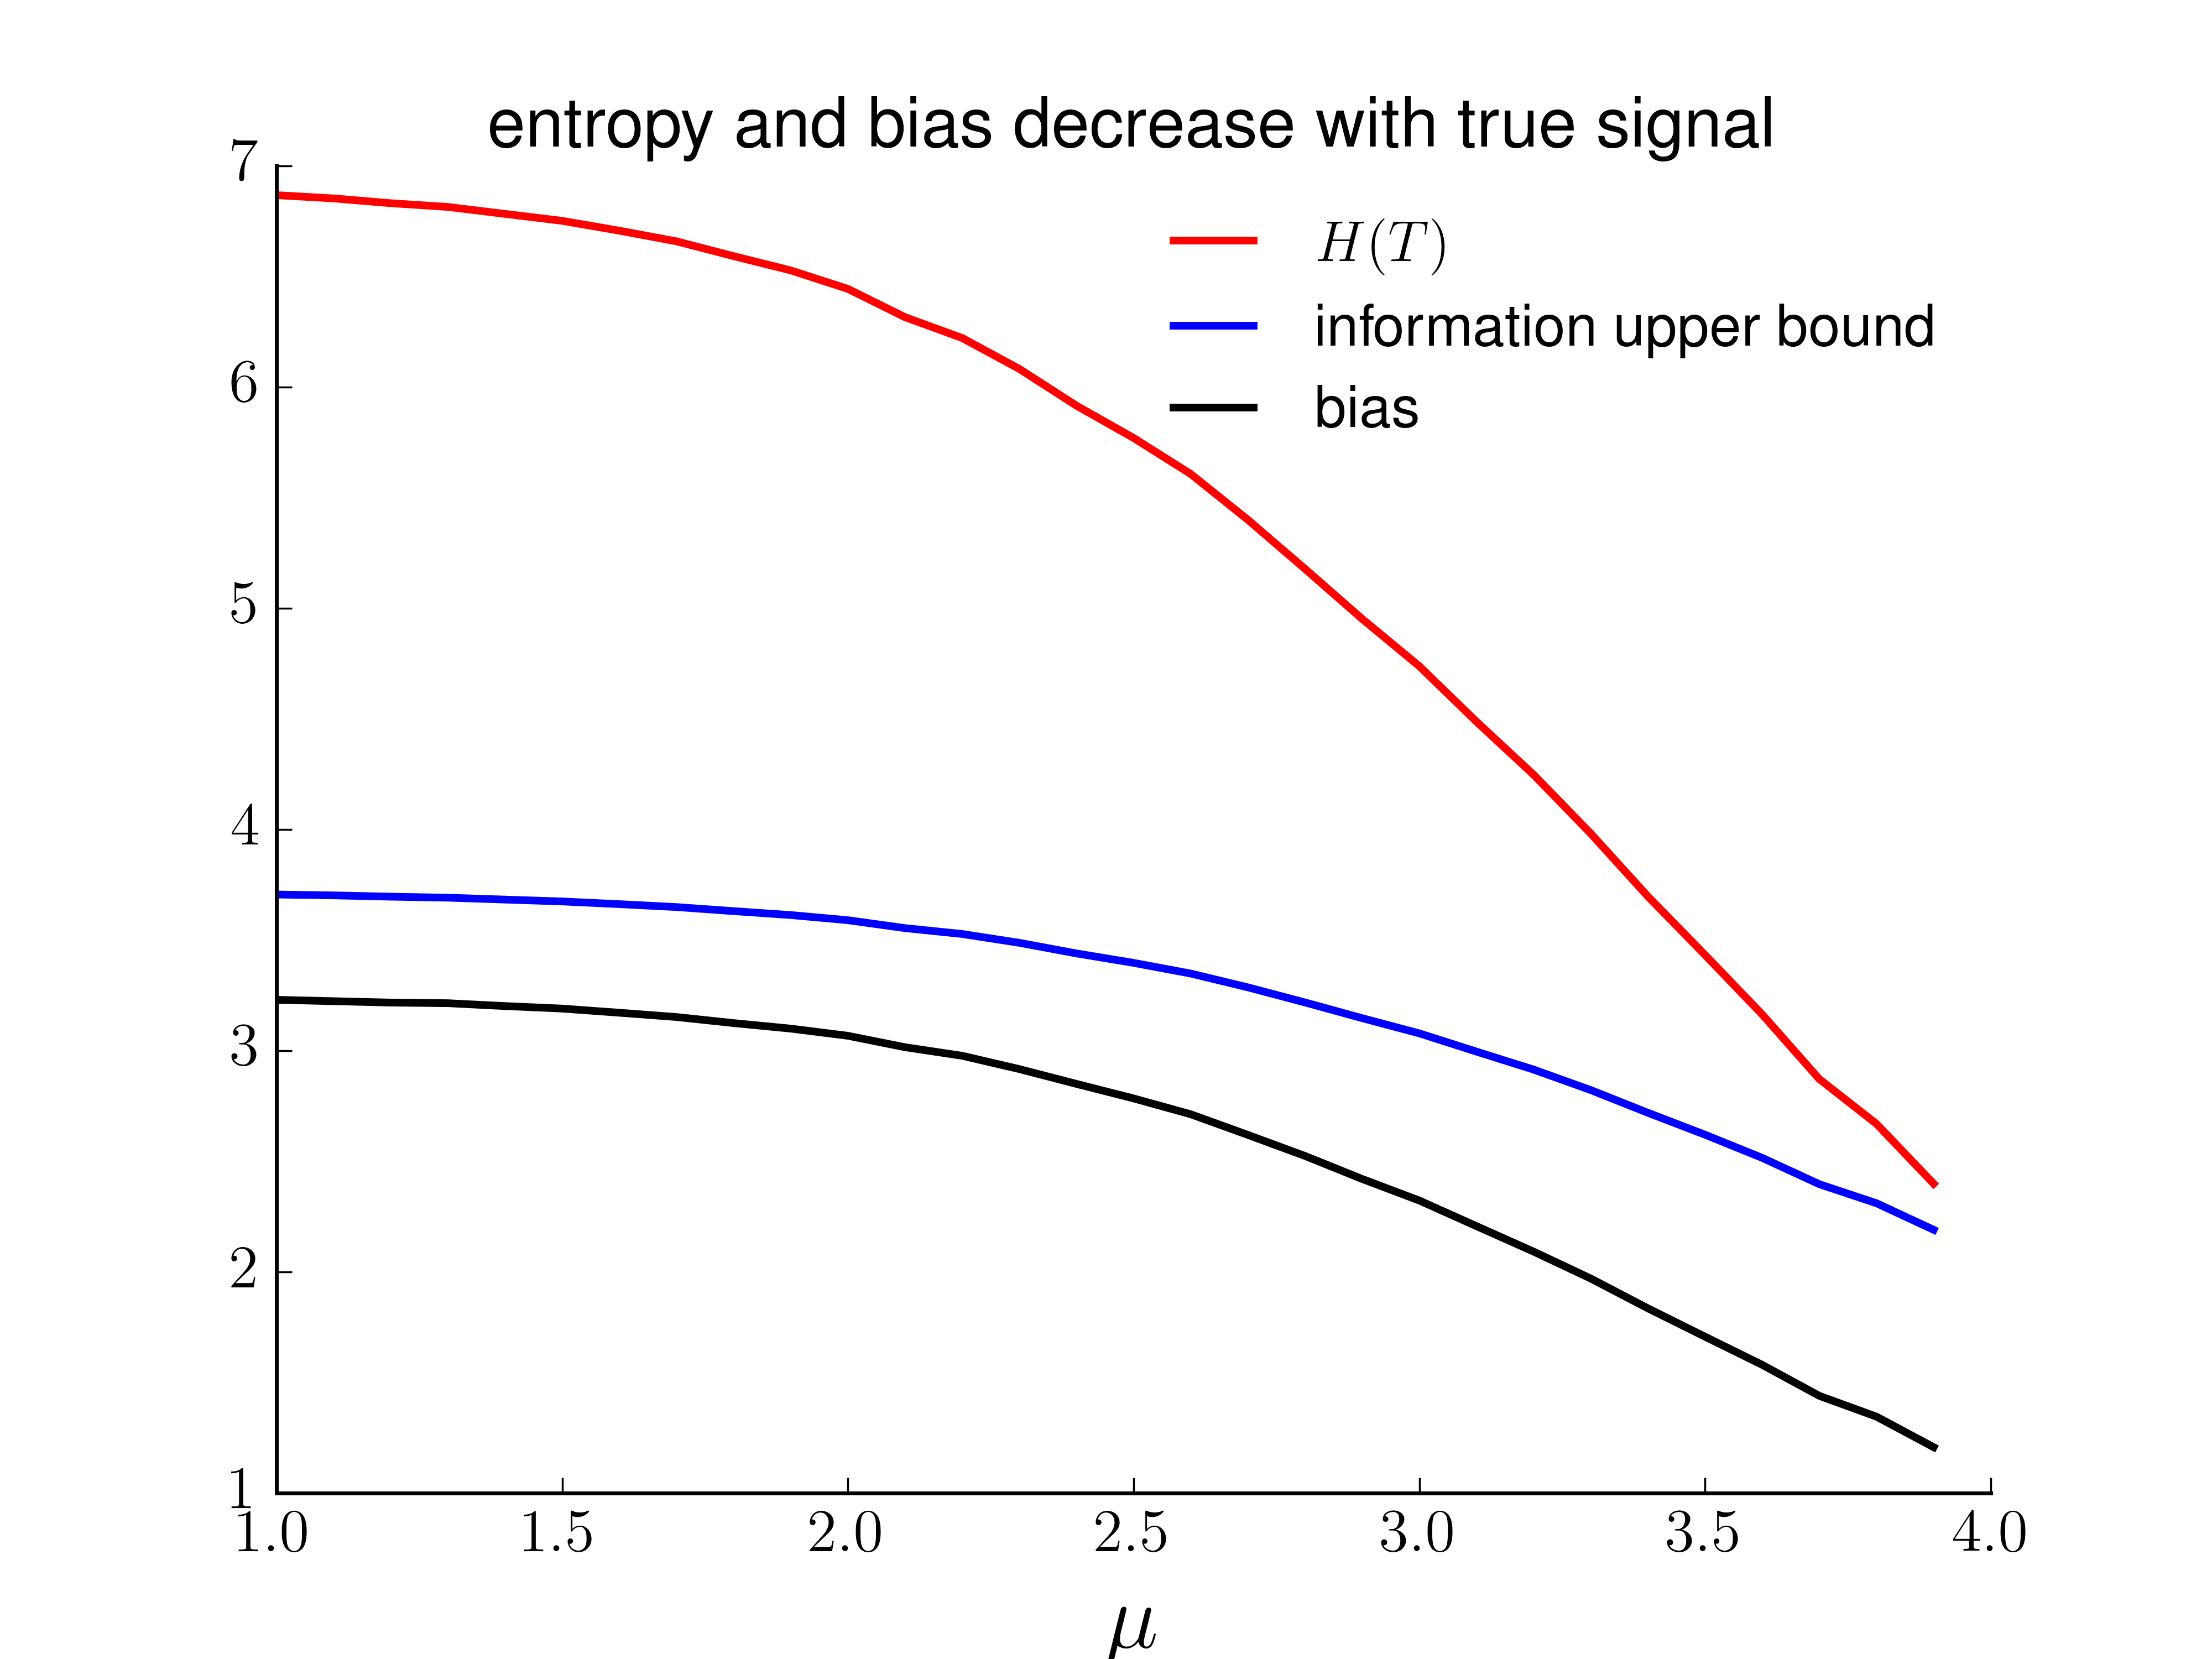
\includegraphics[scale=0.5]{fig_1.png}
		\caption{نمودار میزان سوییدگی 
			$\phi_T$	 
			و کران‌های آن  بر حسب 
			$\mu$}
		\label{simres}
	\end{figure}
	
	\subsection{تفکیک تقریباً مستقل داده‌های غیر
		\lr{i.i.d.}
	}
	
	در این مسئله، تحلیل‌گر داده،
	$n$
	نمونه‌ی زمانی از یک زنجیره‌ی مارکوفی را در اختیار دارد. این تحلیل‌گر قصد دارد از این داده به همان نحوی که از داده‌های 
	\lr{i.i.d.}
	استفاده می‌کند، بهره ببرد. برای این کار، او داده‌ها را به سه قسمت تقسیم می‌کند:
	از 
	$s_1,\dots, s_{n_1}$
	برای انتخاب تحلیل استفاده می‌کند، داده‌‌های
	$s_{n_1},\dots, s_{n_2}$
	را دور می‌اندازد و از
	$s_{n_2},\dots, s_{n}$
	برای تخمین تحلیل انتخاب‌شده با استفاده از بخش اول داده‌ها بهره می‌برد. اگر داده‌ها 
	\lr{i.i.d.}
	می‌بودند، هیچ نشت اطّلاعاتی رخ نمی‌داد و این تحلیل هیچ سوییدگی‌ای ایجاد نمی‌کرد. اما در این حالت که در دیتا روابط زمانی وجود دارد، این گزاره صادق نیست. از نظر شهودی انتظار داریم که اگر
	$n_2 - n_1$
	به قدر کافی بزرگ باشد، سوییدگی تحلیل به قدر دلخواه کم شود.
	
	
	فرض کنید زنجیره‌ی مارکوف ایستان بوده و توزیع ایستان آن را 
	$\mathbf{\pi}$
	بنامید. همچنین فرض کنید:
	\begin{equation}
	\forall \tau \in \mathbb{N} \;\;\;\; \max_s D \Big (\mathbf{P}(s_{\tau} = .| s_1 = s) || \pi \Big) \leq c_0 e^{- c_1 \tau}
	\label{myineq}
	\end{equation}
	یعنی توزیع به شرط حالت اولیه نیز به توزیع ایستان میل می‌کند. از آن‌جایی که این فرآیند، یک فرآیند ایستان است، داریم
	$\mathbf{P}(s_t = s) = \pi$.
	با این فرض و با کمک نامساوی
	\eqref{myineq}
	می‌توان نوشت:
	$$I(s_{t+\tau}; s_t) = \sum_{s} \mathbf{P}(s_t=s) D \Big( \mathbf{P}\big(s_{t+\tau} = .|s_t=s\big) ||\mathbf{P}(s_t=.) \Big) \leq c_0 e^{-c_1\tau}$$
	
	با توجه به نامساوی پردازش اطّلاعات، داریم:
	\begin{flalign}
	I(T;\phi) \leq I(s_1, \dots, s_{n_1} ; s_{n_2+1}, \dots ,s_n)\leq I(s_{n_1}; s_{n_2+1})\leq c_0 e^{-c_1 (n_2-n_1)}
	\end{flalign}
	
	با ترکیب این کران با قضیه‌ی 
	\eqref{mainthm}،
	شهود ما اثبات می‌شود یعنی هر‌چقدر
	$n_2 - n_1$
	بزرگتر باشد، سوییدگی کمتر می‌شود.
	
	
	
	
	
	\section{محدود کردن سوییدگی با تصادفی‌سازی}\label{randomization}
	
	در این بخش، نشان می‌دهیم که حتی اگر فرآیند انتخاب 
	$T$،
	فرآیندی پیچیده بوده و یا ناشناخته باشد، می‌توان با افزودن نویز در مرحله‌ی انتخاب، تا حد زیادی سوییدگی را کم کرد. روش‌های مبتنی بر تصادفی سازی، تاکنون به شدّت در ادبیات یادگیری ماشین و آمار تکرار شده‌اند. در این بخش قصد داریم به تحلیل این روش‌ها بر اساس معیار «اطّلاعات بد» معرفی شده در فصل‌ها بپردازیم.
	
	\subsection{رگولاریزیشن با انتخاب تصادفی}
	
	فرض کنید $m$ تحلیل مختلف
	$\phi_1, \phi_2, \dots, \phi_m$
	در اختیار داریم. قصد داریم تحلیلی را بیابیم که بزرگترین مقدار ممکن را دارد. برای این کار، یک راه اولیه، انتخاب
	$T = \mathrm{argmax}_i \phi_i$
	است. با توجه به 
	\eqref{mainthm}،
	می‌دانیم که اگر 
	$I(T;\phi)$
	کوچک باشد، سوییدگی تخمین کم می‌شود. داریم
	$I(T;\phi) = H(T) - H(T|\phi)$.
	با توجه به این رابطه، به نظر می‌رسد که می‌توان با افزایش 
	$H(T|\phi)$
	یا به عبارتی، تصادفی‌سازی انتخاب 
	$T$،
	میزان سوییدگی را کنترل کرد. با انتخاب 
	$T$
	به صورت تصادفی و مستقل از داده،
	$H(T|\phi)$
	را بیشنه می‌کند، امّا از آن‌جایی که 
	$H(T)$
	را هم زیاد می‌کند، به کمترین
	$I(T;\phi)$
	منتج نمی‌شود. یک ایده این است که علاوه بر افزایش 
	$H(T|\phi)$،
	مقدار
	$\phi_T$
	را هم تا حد امکان بزرگ انتخاب کنیم. بعد از مشاهده‌ی 
	$\phi$
	ها، اندیس 
	$T$
	را به صورت تصادفی و با توزیع 
	$\pi$
	از 
	$\{1, 2, \dots, m\}$
	انتخاب می‌کنیم. از آن‌جا که قصد داریم 
	$\phi_T$
	بزرگ باشد، منطقی است که توزیع 
	$\pi$
	ای را انتخاب کنیم که جواب مسئله‌ی بهینه‌سازی زیر باشد:
	
	\begin{eqnarray*}
		\underset{{ \pi} \in \mathbb{R}^m_+}{\text{maximize}} && H({ \pi}) \\
		\text{to subject } && \sum_{i=1}^{k} \pi_i \phi_i \geq b \mbox{ and }  \sum_{i=1}^{k} \pi_i =1.
	\end{eqnarray*}
	
	شرط
	$\sum_{i = 1}^{k} \pi_i \phi_i \geq b$
	تضمین می‌کند که توزیع انتخاب‌شده به نحوی باشد که به صورت متوسط، مقدار
	$\phi_T$
	بزرگ باشد. این یک مسئله‌ی کلاسیک در تئوری اطّلاعات است و می‌دانیم پاسخ آن، توزیع گیبس است یعنی توزیع
	$\pi^* = Ae^{\beta \phi_i}$.
	در این توزیع، 
	$\beta$
	به نحوی انتخاب شده است که شرط 
	$\sum_{i=1}^{k} \pi_i \phi_i = b$
	برقرار باشد.
	
	اگر دو دیتاست در نظر بگیریم که تنها تفاوت کوچکی با یکدیگر دارند، ممکن است 
	$T = \mathrm{argmax}_i \phi_i$
	در این دو دیتاست تفاوت بزرگی داشته باشد، اما روش تصادفی فوق، احتمالاً جواب‌های نزدیکی را در این دو دیتاست باز خواهد گرداند.
	
	به کمک یک شبیه‌سازی، نشان می‌دهیم این روش از سوییدگی کم می‌کند. فرض کنید دو دسته ‌
	$\phi_i$
	داریم. برای تحلیل‌های 
	$1\leq i\leq N_1$
	داریم
	$\mu_i = \mu >0$
	و برای تحلیل‌های
	$N_1 + 1\leq i \leq m$
	نیز 
	$\mu_i = 0$
	است. در شبیه‌سازی گرفته‌ایم
	$N_1 = 1000$
	و
	$m - N_1 = 100000$،
	یعنی تعداد تحلیل‌ها با میانگین صفر بسیار بیشتر از تعداد تحلیل‌های با میانگین  ناصفر است. مقدار
	$\mu$
	را نیز در بازه‌ی 
	$1$
	تا
	$5$
	تغییر می‌دهیم.  در این تحلیل  به جای گزارش کردم ماکزیمم،
	$K $
	تحلیل با مقدار بزرگتر را گزارش می‌کنیم.  در این شبیه‌سازی به دو کمیت زیر علاقه‌مندیم:
	
	\begin{itemize}
		\item 
		\textbf{	سوییدگی}: $\frac{1}{K} \sum_{i = 1}^{K} \phi_{T_i} - \mu_{T_i}$
		\item
		\textbf{دقّت:}
		$\frac{|\{T_i:T_i\leq N_1\}|}{K}$
	\end{itemize}
	
	نتایج این شبیه‌سازی در نمودار 
	\eqref{sim2}
	آمده است. در این نمودار دیده می‌شود که در رژيم با 
	$\mu$
	کوچک، مطابق انتظار هر دو روش دقّت کمی دارند. در رژیم با 
	$\mu$
	بزرگ، هر دو روش دقتی نزدیک به ۱ دارند ولی روش  تصادفی 
	\lr{Max Entropy}
	سوییدگی کمتری را تجربه کرده است. در رژیم 
	$1<\mu<4$
	روش 
	\lr{Max Entropy}
	خطای بیشتر و در عین حال، سوییدگی کمتری دارد.      
	
	\begin{figure}[h!]
		\centering
		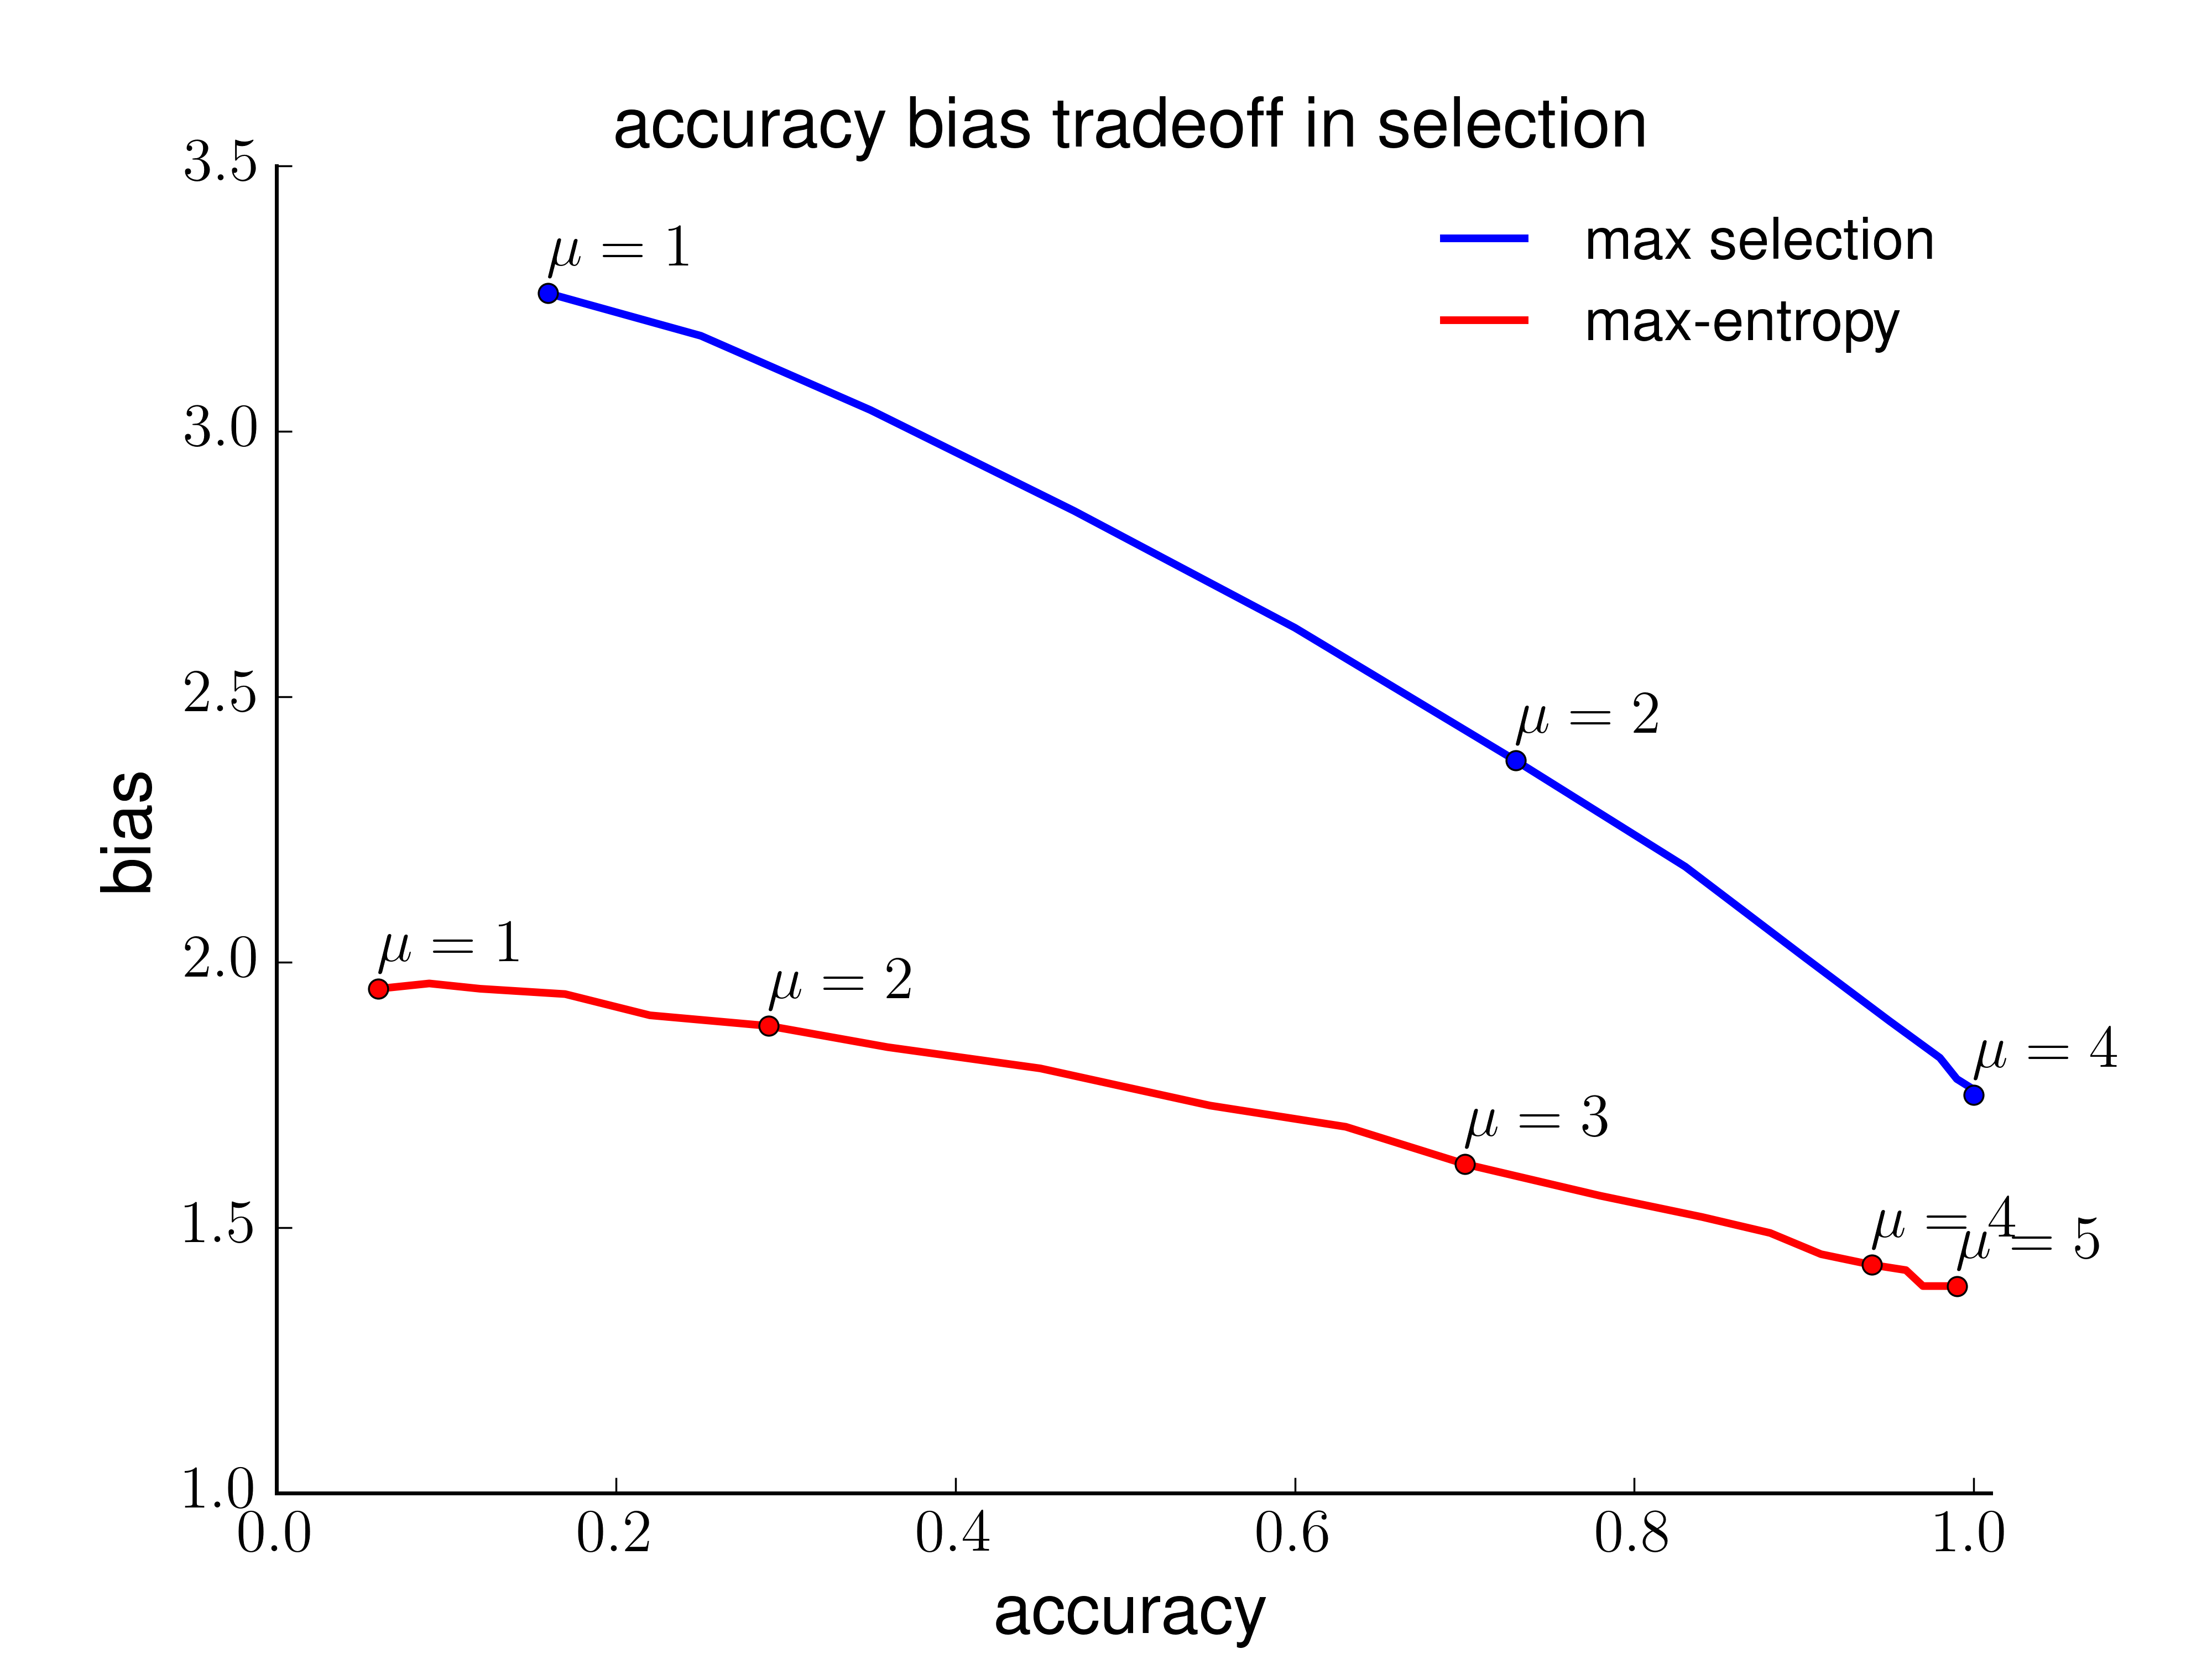
\includegraphics[scale=0.5]{fig_3.png}
		\caption{نتایج شبیه‌‌سازی با تغییر 
			$\mu$	
			با دو روش تصادفی این بخش و روش انتخاب ماکزیمم‌ها
		}
		\label{sim2}
	\end{figure}
	
	\begin{rem}
		توجه نمایید که الگوریتم فوق، لزوماً منجر به کم شدن سوییدگی نمی‌شود، زیرا در عین‌حالی که 
		$H(T|\phi)$
		را افزایش می‌دهد، مقدار
		$H(T)$
		را نیز زیاد می‌کند.
	\end{rem}
	
	\subsection{تصادفی‌سازی در تحلیل‌های چند مرحله‌ای}
	
	
	در ابتدا مدلی از تحلیل داده‌ی تطبیقی ارائه می‌کنیم در آن، تحلیل‌گر داده با انجام آنالیز‌های پی‌در‌پی و استفاده از نتایج آنالیز‌های قبلی، سعی می‌کند به شناختی از داده برسد.
	\begin{itemize}
		\item
		در قدم اول، تحلیل‌گر تابع 
		$\phi_{T_1}$
		را انتخاب می‌کند. نتیجه‌ی این تحلیل 
		$Y_{T_1} \in \R$
		است.
		\item
		در تکرار 
		$k$ ام،
		تحلیل‌گر تابع 
		$\phi_{T_k}$
		را انتخاب می‌کند و در این انتخاب خود، از متغیر‌های
		$$\{Y_{T_1}, Y_{T_2}, \dots, Y_{T_k-1}, T_1, \dots, T_{k-1}\}$$
		استفاده می‌کند.
	\end{itemize}
	
	ما در حالت کلّی اجازه می‌دهیم که نتیجه‌ی آنالیز $k$ام،
	$Y_{T_k}$
	با 
	$\phi_{T_k}$
	متفاوت باشد. به عنوان مثال، ممکن است این نتیجه به صورت
	$Y_{T_k} = \phi_{T_k} + \text{noise}$
	باشد. این سناریو زمانی رخ می‌دهد که تحلیل‌گر داده برای کاستن سوییدگی، به نتایج نویز اصافه کرده و از نتیجه‌ی نویزی در مراحل بعد تحلیل خود استفاده نماید.
	
	در این مدل، بین متغیر‌های مسئله، زنجیره‌ی ماکوف زیر برقرار است:
	$$T_{k+1} - H_k = \{T_1, Y_{T_1}, T_2, Y_{T_2}, \dots, T_k, Y_{T_k}\} - D - \bfphi$$
	
	با نامساوی پردازش اطّلاعات، می‌توان گفت که
	$I(T_{k+1}) \leq I(H_k; \phi)$
	است، بنابراین فرآیندی که در آن اطّلاعات متقابل سابقه و فیدبک سیستم ($H_k$) و نتایج آنالیز‌ها
	$\bfphi$
	کنترل شده باشد، بایاس کمی دارد.
	
	\begin{lem}\label{lem_randomization}
		با تعریف
		$H_k = \{T_1, Y_{T_1}, T_2, Y_{T_2}, \dots, T_k, Y_{T_k}\}$
		داریم:
		$$I(T_{k+1} ; \bfphi) \leq I(H_k;\bfphi) = \sum_{i = 1}^{k} I(Y_{T_i};\phi_{T_i}| H_{i-1}, T_i)$$
	\end{lem}
	از لم
	\eqref{lem_randomization}
	می‌توان دریافت که با محدودکردن
	\lr{$I(Y_{T_i};\phi_{T_i}| H_{i-1}, T_i)$}
	در هر مرحله، می‌توان 
	\lr{$I(T_{k+1} ; \bfphi)$}
	را کنترل کرد. در نتیجه انگار یک «بودجه‌ی اطّلاعات استفاده‌شده» مانند
	\lr{$I_b$}
	داریم که در هر مرحله، تحلیل‌گر برای انتخاب اندیس فعلی بر اساس اندیس‌های قبلی از آن خرج می‌کند. در نتیجه فرآیند را می‌توان تا جایی ادامه داد که بودجه تمام شود.
	
	اگر بتوانیم در هر مرحله، 
	\lr{$I(Y_{T_i};\phi_{T_i}| H_{i-1}, T_i)$}
	را کم کنیم، می‌توان تعداد مراحل بیشتری را پیمود. یک راه برای دستیابی به این هدف، اضافه‌کردن نویز گاوسی است. فرض کنید
	\lr{$\phi_i\sim \Nd(\mu_i,\frac{\sigma^2}{n})$}
	و برای هر
	\lr{$k$}،
	\lr{$(\phi_1,\cdots,\phi_k)$}
	مشترکاً گاوسی باشند. همچنین فرض کنید که در 
	\lr{$j$}امین
	مرحله، داریم
	\lr{$Y_{T_j}=\phi_{T_j} + W_j$}
	که
	\lr{$W_j$}ها
	مستقلند و داریم
	\lr{$W_j\sim\Nd(0,\frac{\omega_j^2}{n})$}
	
	در این حالت می‌توان
	\lr{$\E\left[|Y_{T_{k+1}} - \mu_{T_{k+1}}|\right]$}
	را محدود کرد.
	\begin{thm}\label{thm_randgaussian}
		فرض کنید
		\lr{$\phi_i\sim \Nd(\mu_i,\frac{\sigma^2}{n})$}
		و برای هر
		\lr{$k$}،
		\lr{$(\phi_1,\cdots,\phi_k)$}
		مشترکاً گاوسی باشند. همچنین فرض کنید که به ازای هر
		\lr{$j$}،
		داریم
		\lr{$Y_{T_j}=\phi_{T_j} + W_j$}
		که
		\lr{$W_j$}ها
		مستقلند و داریم
		\lr{$W_j\sim\Nd(0,\frac{\sigma^2\sqrt{j}}{n})$}.
		در این صورت برای هر
		\lr{$k\in\mathcal{N}$}
		داریم:
		\begin{equation}
		\E\left[|Y_{T_{k+1}} - \mu_{T_{k+1}}|\right] \leq c\left(\frac{\sigma k^{\frac{1}{4}}}{n^{\frac{1}{2}}}\right)
		\end{equation}
		که
		\lr{$c$}
		یک ثابت است و مستقل از 
		\lr{$\sigma, k, n$}.
	\end{thm}
اگر دنباله‌ی 
$(T_1, T_2, \dots)$
به صورت غیر تطبقی تولید می‌شدند و نویزی نیز اضافه نمی‌شد، به کران
$\E[|Y_{T_{k+1}} - \mu_{T_{k+1}}|] \leq \frac{\sigma}{n}$
می‌رسیدیم. در مدل تطیقی و در مراحل ابتدایی نیز می‌توانستیم به این سوییدگی برسیم، اما به مرور میزان سوییدگی افزایش پیدا می‌کرد. ضریب 
 $k^\frac{1}{4}$
 را می‌توان به عنوان هزینه‌ی پردازش تطبیقی در نظر گرفت. در این‌جا ذکر این نکته جالب است که می‌توان مثال‌هایی تطبیقی یافت که بدون افزودن نویز، در آن‌ها سوییدگی از حالت غیر تطبیقی بیشتر است، یعنی
$\E[|Y_{T_{k+1}} - \mu_{T_{k+1}}|] = \Omega(\sigma \frac{k}{n})$.


\section{پیشنهاد برای کار‌های آتی}
برای انجام کار‌های آتی چندین مسیر امیدوار‌کننده به نظر می‌رسد که در این بخش، به صورت اجمالی به آن‌ها اشاره می‌کنیم.
\begin{itemize}
	\item 
در مدل‌سازی این مقاله، تحلیل‌گر داده همواره تنها یک تابع را بر می‌گزیند و مقدار آن را گزارش می‌کند. در کاربرد‌‌های تجربی، بسیار پیش‌ می‌آید که تعدادی تحلیل انتخاب شده و نتایج آن گزارش شوند. به عنوان مثال، ممکن است این تعداد با توجه به داده، تعداد تحلیل‌های جالب مشخص شود. این انتخاب تصادفی تعداد داده‌های گزارش شده نیز می‌تواند باعث نشر «اطّلاعات بد» از دیتاست شده و باعث افزایش سوییدگی گردد. تعمیم چهارچوب مطرح شده در این مقاله برای حالتی که تحلیل‌گر تعدادی تحلیل را گزارش می‌کند و خود این تعداد نیز یک متغیر تصادفی است، از اهمیت تجربی و تئوری بالایی برخوردار است.

\item
در این مقاله و در مدل‌سازی تحلیل تطبیقی داده‌ها، همواره فرض بر این است که دیتاست در طول زمان ثابت است. این فرض در بسیاری از کاربرد‌ها از واقعیّت به دور است. فرض بهتر این است که خود دیتاست نیز ماتریسی ‌تصادفی در نظر گرفته‌شود که در طول زمان در حال تغییر است. مبه عنوان مثال، این ماتریس می‌توان یک فرآیند تصادفی مارکوف را تشکیل دهد. مدل‌سازی مسئله در این شرایط و با اعمال محدودیت‌هایی از تغییرات ممکن در دیتاست، می‌تواند به نتایج بسیار با اهمیتی منجر شود. در این مدل جدید می‌توان به بررسی این موضوع پرداخت که استفاده داده‌های دیتاست در بخش از زمان‌ها  برای انتخاب تحلیل و استفاده از زمان‌هایی دیگر برای تخمین آن، به چه میزان می‌تواند ایجاد سوییدگی کند.

\item
در مدل تحلیل تطبیقی داده، به خصوص در مثال متغیر‌های گاوسی، برای ارائه‌ی کران سوییدگی، توزیع نویز به نحوی انتخاب‌شده که محاسبات ساده گردند. پیدا‌کردن توزیع‌های نویزی که منجر به کوچکترین سوییدگی شوند می‌تواند بسیار جالب و کاربردی باشد.

\item 
در تئوری یادگیری ماشیمن، الگوریتم‌های آنلاین متعددی وجود دارند که به صورت «تطبیقی» به پردازش داده‌ها می‌پردازند. چهارچوب فعلی می‌تواند به عنوان ابزاری نیرومند برای تحلیل بایاس‌های چنین الگوریتم‌های به کار رود.
\end{itemize}

	\bibliographystyle{ieeetr-fa}
	\bibliography{references}
	\clearpage
	\appendix
	\section{پیش‌نیازهای موردنیاز جهت فهم اثبات‌های قضایا}\label{pre_requirements}
	\subsection{متغیّرهای تصادفی زیر--گاوسی}
	\begin{den}
		متغیّر تصادفی
		\lr{$X$}
		با میانگین
		\lr{$\mu = \mathbb{E}[X]$}
		را زیر--گاوسی می‌نامیم هرگاه عدد مثبتی مانند
		\lr{$\sigma$}
		وجود داشته باشد، به قسمی که برای هر
		\lr{$\lambda\in\mathbb{R}$}
		داشته باشیم:
		\[\E\left[e^{\lambda(X-\mu)}\right]\leq e^{\frac{\sigma^2\lambda^2}{2}}\]
	\end{den}
	ثابت
	\lr{$\sigma$}
	را پارامتر این متغیّر تصادفی می‌نامیم. به عنوان مثال، یک متغیّر تصادفی گاوسی با واریانس
	\lr{$\sigma^2$}،
	خود یک متغیّر تصادفی زیر--گاوسی با پارامتر
	\lr{$\sigma$}
	است. هم‌چنین تعداد زیادی از متغیّرهای تصادفی غیر گاوسی، زیر--گاوسی هستند.
	
	\begin{thm}	\label{thm1subgaussian}
		برای هر متغیّر تصادفی زیر--گاوسی 
		\lr{$X$}
		با متوسّط
		\lr{$\mu = \E[X]$}
		و پارامتر
		\lr{$\sigma$}
		داریم:
		\begin{equation}
		\Prob[|X-\mu|\geq t] \leq 2e^{-\frac{t^2}{2\sigma^2}}
		\end{equation}
	\end{thm}
	\begin{proof}
		از نامساوی مارکف می‌دانیم:
		\[\Prob[X-\mu\geq t] = \Prob[e^{\lambda (X-\mu)} \geq e^{\lambda t}] \leq \frac{\E\left[e^{\lambda (X-\mu)}\right]}{e^{\lambda t}} \]
		حال با توجّه به تعریف متغیّرهای تصادفی زیر--گاوسی داریم:
		\[\Prob[X-\mu\geq t] \leq \frac{\E\left[e^{\lambda (X-\mu)}\right]}{e^{\lambda t}} \leq \exp(\frac{\sigma^2\lambda^2}{2} - \lambda t)\]
		نامساوی بالا به ازای هر
		\lr{$\lambda\in\R$}
		برقرار است، من‌جمله
		\lr{$\lambda$}ای
		که طرف راست را کمینه کند. در نتیجه:
		\begin{equation}
		\Prob[X-\mu\geq t] \leq \inf_\lambda\left\{\exp(\frac{\sigma^2\lambda^2}{2} - \lambda t) \right\} = e^{-\frac{t^2}{2\sigma^2}}
		\end{equation}
		همچنین اگر متغیّر تصادفی
		\lr{$X$}،
		زیر--گاوسی باشد، 
		\lr{$-X$}
		هم زیر--گاوسی است و به طور مشابه، داریم:
		\[\Prob[-X+\mu\geq t] = \Prob[X-\mu\leq -t]\leq  e^{-\frac{t^2}{2\sigma^2}}\]
		و می‌توان نوشت:
		\[\Prob[|X-\mu|\geq t] \leq \Prob[X-\mu\geq t] + \Prob[X-\mu\leq -t] \leq 2e^{-\frac{t^2}{2\sigma^2}}\]
	\end{proof}
	
	متغیّرهای تصادفی زیر--گاوسی خواصّ گوناگونی دارند، تعدادی از این خواص را در قضایای بعدی مشاهده می‌کنیم.
	
	\begin{thm}\label{thm2subgaussian}
		فرض کنید 
		\lr{$X$}
		یک متغیّر تصادفی زیر--گاوسی با امید ریاضی
		\lr{$\E[X]=0$}
		باشد، در این صورت اگر متغیّر تصادفی 
		\lr{$Z$}
		را به صورت
		\lr{$Z\sim \Nd(0,2\sigma^2)$}
		در نظر بگیریم، داریم:
		\begin{equation}
		\Prob[|X|\geq s] \leq \sqrt{8}e \Prob[|Z|\geq s] \qquad \forall s \geq 0
		\label{thm2eq}
		\end{equation}
	\end{thm}
	\begin{proof}
		از قضیه‌ی
		\ref{thm1subgaussian}
		داریم:
		\[\Prob[X\geq t] \leq e^{-\frac{t^2}{2\sigma^2}}\qquad \forall t\geq0\]
		و از طرف دیگر، با توجّه به کران
		\lr{Mills ratio}
		برای توزیع‌های گاوسی داریم:
		\[\Prob[Z\geq t] \geq\left(\frac{\sqrt{2}\sigma}{t} - \frac{(\sqrt{2}\sigma)^3}{t^3} \right) e^{-\frac{t^2}{4\sigma^2}}\]
		حال دو حالت زیر را در نظر می‌گیریم:	
		حالتی که 
		\lr{$t\in[0,2\sigma]$}
		باشد. در این حالت، داریم:
		\[\Prob[Z\geq t] \geq \Prob[Z\geq 2\sigma] = \left(\frac{1}{\sqrt{2}} - \frac{1}{2\sqrt{2}} \right) e^{-1} = \frac{1}{\sqrt{8}e}\]
		و از آن‌جا که
		\lr{$\Prob[X\geq t] \leq 1$}،
		داریم:
		\[\frac{\Prob[X\geq t]}{\Prob[Z\geq t]} \leq \sqrt{8}e\]
		
		
		حالتی که
		\lr{$t>2\sigma$}
		باشد. در این حالت اگر کران
		\lr{Mills ratio}
		را با کران به دست آمده در قضیه‌ی
		\ref{thm1subgaussian}
		ترکیب کنیم و تعریف کنیم
		\lr{$s = \frac{t}{\sigma}$}،
		داریم:
		\begin{flalign*}
		\sup_{t>2\sigma} \frac{\Prob[X\geq t]}{\Prob[Z\geq t]} &\leq \sup_{s>2}\frac{e^{-\frac{s^2}{4}}}{\frac{\sqrt{2}}{s} - \frac{2\sqrt{2}}{s^3}}\\
		&\leq \sup_{s>2} s^3 e^{-\frac{s^2}{4}}\\
		&\leq \sqrt{8}e
		\end{flalign*}
		پس در هر دو حالت نامساوی
		(\ref{thm2eq})
		برقرار است.		
	\end{proof}
	\begin{thm}\label{thm3subgaussian}
		فرض کنید 
		\lr{$X$}
		یک متغیّر تصادفی با امید ریاضی
		\lr{$\E[X]=0$}
		باشد و بتوانیم عدد ثابتی مانند
		\lr{$c$}
		و یک متغیّر تصادفی
		\lr{$Z\sim\Nd(0,\tau^2)$}
		بیابیم، به قسمی که
		\begin{equation}
		\Prob[|X|\geq s] \leq c \Prob[|Z|\geq s] \qquad \forall s \geq 0
		\end{equation}
		در این صورت ثابتی مانند
		\lr{$\theta\geq0$}
		وجود دارد، به گونه‌ای که:
		\begin{equation}
		\E\left[X^{2k}\right] \leq \frac{(2k)!}{2^kk!}\theta^{2k}\qquad \forall k \in \mathbb{N}
		\end{equation}
	\end{thm}
	\begin{proof}
		اگر 
		\lr{$Z \sim \mathcal{N}(0,\tau^2)$}
		و
		\lr{$X$}
		یک متغیّر تصادفی باشد که در رابطه‌ی
		\lr{$\Prob[|X|\geq s] \leq c \Prob[|Z|\geq s]$}
		به ازای هر
		\lr{$s\geq0$}
		صدق کند، با توجّه به این‌که 
		\lr{$X^{2k}$}
		یک متغیّر تصادفی نامنفی است، می‌توان نوشت:
		\begin{flalign*}
		\E\left[X^{2k}\right] &= \int_{0}^{+\infty}\Prob[X^{2k}>s]ds\\
		&= \int_{0}^{+\infty}\Prob[|X|>s^{\frac{1}{2k}}]ds\\
		&\leq c \int_{0}^{+\infty}\Prob[|Z|>s^{\frac{1}{2k}}]ds\\
		&= c \E\left[Z^{2k}\right]
		\end{flalign*}
		و از آن‌جا که متغیّر تصادفی
		\lr{$Z$}،
		گاوسی است، می‌دانیم:
		\[ \E\left[Z^{2k}\right] = \frac{(2k)!}{2^kk!} \tau^{2k} \qquad \forall k\in \N\]
		در نتیجه:
		\begin{flalign*}
		\E\left[X^{2k}\right] &\leq c \E\left[Z^{2k}\right]\\
		&= c \frac{(2k)!}{2^kk!} \tau^{2k}\\
		&\leq \frac{(2k)!}{2^kk!} (c\tau)^{2k}
		\end{flalign*}
		در نتیجه اگر قرار دهیم
		\lr{$\theta = c\tau$}
		به حکم می‌رسیم.
	\end{proof}
	\begin{thm}\label{thm4subgaussian}
		فرض کنید 
		\lr{$X$}
		یک متغیّر تصادفی با امید ریاضی
		\lr{$\E[X]=0$}
		باشد و ثابتی مانند
		\lr{$\theta \geq 0$}
		وجود داشته باشد، به قسمی که:
		\begin{equation}
		\E\left[X^{2k}\right] \leq \frac{(2k)!}{2^kk!}\theta^{2k}\qquad \forall k \in \mathbb{N}
		\end{equation}
		در این صورت متغیّر تصادفی
		\lr{$X$}،
		زیرگاوسی با پارامتر
		\lr{$\sigma = \theta\sqrt{2}$}
		است.
	\end{thm}
	\begin{proof}
		به ازای هر
		\lr{$\lambda\in\R$}
		داریم:
		\[\E\left[e^{\lambda X}\right] \leq 1 + \sum_{k=2}^{\infty} \frac{|\lambda|^k\E\left[|X|^k\right]}{k!}\]
		(جمله‌ی متناظر با
		\lr{$k=1$}
		به دلیل این‌که
		\lr{$\E[X]=0$}
		حذف شده است) اگر 
		\lr{$X$}
		حول صفر تقارن داشته باشد، جملات دارای
		\lr{$k$}
		فرد از بین می‌روند و داریم:
		\[\E\left[e^{\lambda X}\right] \leq 1 + \sum_{k=1}^{\infty} \frac{\lambda^(2k)\E\left[|X|^k\right]}{(2k)!}\frac{(2k)!\theta^{2k}}{2^kk!} = e^{\frac{\lambda^2\theta^2}{2}}\]
		که نتیجه می‌دهد 
		\lr{$X$}
		یک متغیّر تصادفی زیر--گاوسی با پارامتر
		\lr{$\theta$}
		است.
		
		\noindent
		اگر
		\lr{$X$}
		متقارن نباشد، می‌توانیم یک کران بالا برای جملات مربوط به 
		\lr{$k$}های
		فرد بیابیم:
		\begin{flalign*}
		\E\left[|\lambda X|^{2k+1}\right]&\leq\sqrt{\E\left[|\lambda X|^{2k}\right]\E\left[|\lambda X|^{2k+2}\right]}\\
		&\leq \frac{1}{2}\left(\lambda^{2k}\E\left[X^{2k}\right] + \lambda^{2k+2}\E\left[X^{2k+2}\right]\right)
		\end{flalign*}
		(نامساوی اوّل از نامساوی کوشی-شوارتز نتیجه می‌شود و نامساوی دوم از نامساوی میانگین حسابی--هندسی.) در نتیجه داریم:
		\begin{flalign*}
		\E\left[|\lambda X|^{2k+1}\right] &\leq 1 + \left(\frac{1}{2}+\frac{1}{2\times3!}\right)\lambda^2\E\left[X^2\right] +\\
		&+ \sum_{k=2}^{\infty} \left(\frac{1}{(2k)!} + \frac{1}{2}\left[\frac{1}{(2k-1)!} + \frac{1}{(2k+1)!}\right]\right)\lambda^{2k}\E\left[X^{2k}\right]\\
		&\leq \sum_{k=0}^{\infty} 2^k\frac{\lambda^{2k} \E\left[X^{2k}\right]}{(2k)!}\\
		&\leq \sum_{k=0}^{\infty} 2^k\frac{\lambda^{2k}}{(2k)!} \frac{(2k)!\theta^{2k}}{2^kk!}\\
		&= \exp(\frac{(\sqrt{2}\lambda\theta)^2}{2})
		\end{flalign*}
		که نتیجه می‌دهد 
		\lr{$X$}
		یک متغیّر تصادفی زیر--گاوسی با پارامتر
		\lr{$\theta\sqrt{2}$}
		است.
	\end{proof}
	
	\begin{thm}\label{thm5subgaussian}
		فرض کنید 
		\lr{$X$}
		یک متغیّر تصادفی با امید ریاضی
		\lr{$\E[X]=0$}
		باشد و بتوانیم عدد ثابتی مانند
		\lr{$c$}
		و یک متغیّر تصادفی
		\lr{$Z\sim\Nd(0,\tau^2)$}
		بیابیم، به قسمی که
		\begin{equation}
		\Prob[|X|\geq s] \leq c \Prob[|Z|\geq s] \qquad \forall s \geq 0
		\end{equation}
		در این صورت 
		\lr{$X$}
		یک متغیّر تصادفی زیر--گاوسی با پارامتر
		\lr{$\sqrt{2}c\tau$}
		است.
	\end{thm}
	\begin{proof}
		با توجّه به اینکه
		\[\Prob[|X|\geq s] \leq c \Prob[|Z|\geq s] \qquad \forall s \geq 0\]
		با استفاده از قضیه‌ی
		\ref{thm3subgaussian}
		داریم:
		\[\E\left[X^{2k}\right] \leq \frac{(2k)!}{2^kk!}\theta^{2k}\qquad \forall k \in \mathbb{N}\]
		که 
		\lr{$\theta = c\tau$}.
		حال با توجّه به قضیه‌ی
		\ref{thm4subgaussian}
		می‌توانیم نتیجه بگیریم که متغیّر تصادفی
		\lr{$X$}،
		یک متغیّر تصادفی زیر--گاوسی با پارامتر
		\lr{$\sigma = \sqrt{2}\theta = \sqrt{2} c\tau$}
		است.
	\end{proof}
	
	\begin{thm}\label{thm6subgaussian}
		فرض کنید 
		\lr{$X$}
		یک متغیّر تصادفی زیر--گاوسی با امید ریاضی
		\lr{$\E[X]=0$}
		و پارامتر
		\lr{$\sigma$}
		باشد، در این صورت:
		\begin{equation}
		\E\left[e^{\frac{s X^2}{2\sigma^2}}\right] \leq \frac{1}{\sqrt{1-s}}\qquad \forall s \in [0,1)
		\end{equation}
	\end{thm}
	\begin{proof}
		درستی حکم برای 
		\lr{$s=0$}
		واضح است. برای 
		\lr{$s\in(0,1)$}،
		از آن‌جا که 
		\lr{$X$}
		یک متغیّر تصادفی زیر--گاوسی است، داریم:
		\[\E\left[e^{\lambda X}\right]\leq e^{\frac{\lambda^2\sigma^2}{2}}\]
		دو طرف نامساوی فوق را در 
		\lr{$e^{-\frac{\lambda^2\sigma^2}{2s}}$}
		ضرب می‌کنیم:
		\[\E\left[e^{\lambda X - \frac{\lambda^2\sigma^2}{2s}}\right]\leq e^{\frac{\lambda^2\sigma^2(s-1)}{2s}}\]
		از آن‌جا که رابطه‌ی اخیر به ازای هر
		\lr{$\lambda\in\R$}
		برقرار است، می‌توانیم از دوطرف آن روی
		\lr{$\lambda$}
		انتگرال بگیریم. انتگرال سمت راست نامساوی عبارت است از:
		\[\int_{-\infty}^{\infty} \exp\left(\frac{\lambda^2\sigma^2(s-1)}{2s}\right)d\lambda = \frac{1}{\sigma}\sqrt{\frac{2\pi s}{1-s}}\]
		و انتگرال سمت چپ نامساوی:
		\begin{flalign*}
		\int_{-\infty}^{\infty} \E\left[e^{\lambda X - \frac{\lambda^2\sigma^2}{2s}}\right] d\lambda &= \E\left[\int_{-\infty}^{\infty} e^{\lambda X - \frac{\lambda^2\sigma^2}{2s}} d\lambda\right]\\
		&= \E\left[\frac{\sqrt{2\pi s}}{\sigma}e^{\frac{sX^2}{2\sigma^2}}\right]\\
		&= \frac{\sqrt{2\pi s}}{\sigma} \E\left[e^{\frac{sX^2}{2\sigma^2}}\right]
		\end{flalign*}
		در نتیجه:
		\begin{flalign*}
		\E\left[e^{\frac{sX^2}{2\sigma^2}}\right] &= \frac{\sigma}{\sqrt{2\pi s}} \int_{-\infty}^{\infty} \E\left[e^{\lambda X - \frac{\lambda^2\sigma^2}{2s}}\right] d\lambda\\
		&\leq \frac{\sigma}{\sqrt{2\pi s}} \int_{-\infty}^{\infty} \exp\left(\frac{\lambda^2\sigma^2(s-1)}{2s}\right)d\lambda\\
		&= \frac{\sigma}{\sqrt{2\pi s}} \frac{1}{\sigma}\sqrt{\frac{2\pi s}{1-s}}\\
		&= \frac{1}{\sqrt{1-s}}
		\end{flalign*}
	\end{proof}
	
	\subsection{متغیّرهای تصادفی زیر--نمایی}
	\begin{den}
		متغیّر تصادفی
		\lr{$X$}
		با امید ریاضی
		\lr{$\mu = \E[X]$}
		را زیر--نمایی می‌نامیم اگر پارامترهای نامنفی
		\lr{$(\nu,\alpha)$}
		وجود داشته باشند، به قسمی که برای هر
		\lr{$\lambda$}
		که
		\lr{$|\lambda|<\frac{1}{\alpha}$}
		داشته باشیم:
		\[\E\left[e^{\lambda(X-\mu)}\right]\leq e^{\frac{\nu^2\lambda^2}{2}}\]
	\end{den}
	از تعریف متغیّرهای تصادفی زیر--گاوسی و زیر--نمایی می‌توان نتیجه گرفت که هر متغیّر تصادفی زیر--گاوسی با پارامتر
	\lr{$\sigma$}
	زیر--نمایی هم هست با پارامترهای
	\lr{$\nu=\sigma$}
	و
	\lr{$\alpha = 0$}،
	ولی عکس آن الزاماً درست نیست.
	
	می‌توان قضیه‌ای مشابه قضیه‌ی
	\ref{thm1subgaussian}
	برای متغیّرهای تصادفی زیر--نمایی بیان کرد:
	\begin{thm}\label{thm1subexponential}
		برای هر متغیّر تصادفی زیر--نمایی با متوسّط
		\lr{$\mu = \E[X]$}
		و پارامترهای
		\lr{$\nu,\alpha$}
		داریم:
		\begin{equation}
		\Prob[X-\mu\geq t] \leq \begin{cases}
		e^{-\frac{t^2}{2\nu^2}} &  0\leq t \leq \frac{\nu^2}{\alpha}\\
		e^{-\frac{t}{2\alpha}} &  t>\frac{\nu^2}{\alpha}\\
		\end{cases}
		\end{equation}
	\end{thm}
	\begin{proof}
		از نامساوی مارکف می‌دانیم:
		\[\Prob[X-\mu\geq t] = \Prob[e^{\lambda(X-\mu)}\geq e^{\lambda t}] \leq \frac{\E\left[e^{\lambda(X-\mu)}\right]}{e^{\lambda t}}\]
		و در نتیجه با استفاده از تعریف متغیّرهای تصادفی زیر--نمایی می‌توان نوشت:
		\[\Prob[X-\mu\geq t] \leq \frac{\E\left[e^{\lambda(X-\mu)}\right]}{e^{\lambda t}} \leq \exp(\frac{\nu^2\lambda^2}{2} - \lambda t) \qquad \forall \lambda\in[0,\frac{1}{\alpha})\]
		حال می‌خواهیم مقدار کمینه‌ی عبارت
		\lr{$g(\lambda,t) = \frac{\nu^2\lambda^2}{2} - \lambda t$}
		را محاسبه کنیم. مقدار کمینه‌ی این عبارت در
		\lr{$\lambda^* = \frac{t}{\nu^2}$}
		رخ می‌دهد. اگر داشته باشیم
		\lr{$\frac{t}{\nu^2}\in[0,\frac{1}{\alpha})$}
		و به تبع آن
		\lr{$0\leq t\leq \frac{\nu^2}{\alpha}$}،
		می‌توانیم
		\lr{$\lambda^*$}
		را به جای
		\lr{$\lambda$}
		قرار دهیم و در این صورت داریم:
		\[\Prob[X-\mu\geq t]\leq e^{-\frac{t^2}{2\nu^2}}\]
		اگر 
		\lr{$t>\frac{\nu^2}{\alpha}$}
		باشد، از آن‌جا که تابع
		\lr{$g(.,t)$}
		در بازه‌ی
		\lr{$[0,\lambda^*]$}
		به طور یکنوا کاهشی است، مقدار کمینه‌ی آن در مرز
		\lr{$\lambda = \frac{1}{\alpha}$}
		رخ می‌دهد، در نتیجه:
		\[\Prob[X-\mu\geq t]\leq e^{-\frac{t}{\alpha} + \frac{1}{2\alpha}\frac{\nu^2}{\alpha}} \leq e^{-\frac{t}{\alpha} + \frac{1}{2\alpha}t} = e^{-\frac{t}{2\alpha}} \]
	\end{proof}
	
	\subsection{بیان دیگری از فاصله‌ی
		\lr{KL}}
	می‌دانیم فاصله‌ی
	\lr{KL}
	به صورت زیر تعریف می‌شود:
	\begin{equation}
	D_{KL}(p||q) = \sum_{x\in \mathcal{X}} p(x)\ln(\frac{p(x)}{q(x)})
	\end{equation}
	تعریف معادلی برای فاصله‌ی
	\lr{KL}
	در قضیه‌ی زیر بیان شده است:
	\begin{thm}\label{thm_kldiv}
		فرض کنید 
		\lr{$p(x)$}
		و
		\lr{$q(x)$}
		دو توزیع روی الفبای یکسان
		\lr{$\mathcal{X}$}
		باشند. در این صورت می‌توان نوشت:
		\begin{equation}
		D_{KL}(p||q) = \sup_f \left\{\E_p[f(X)] - \ln \E_q[e^{f(X)}]\right\}
		\end{equation}
		که سوپریمم روی همه‌ی توابع
		\lr{$f$}
		گرفته می‌شود که در آن‌ها
		\lr{$\E_p[f(X)]$}
		و
		\lr{$\E_q[e^{f(X)}]$}
		خوش‌تعریف باشند.
	\end{thm}
	\subsubsection{اثبات قضیه‌ی
		\eqref{thm_kldiv}}
	\begin{proof}
		ابتدا فرض کنید تابع
		\lr{$f$}
		را به این صورت تعریف کنیم:
		\[f(x) = \ln(\frac{p(x)}{q(x)}).\]
		در این حالت مشاهده می‌کنیم که:
		\begin{flalign*}
		\E_p[f(X)] - \ln \E_q[e^{f(X)}] &= \sum_{x\in \mathcal{X}} p(x)\ln(\frac{p(x)}{q(x)}) - \ln(\sum_{x\in \mathcal{X}}q(x) \frac{p(x)}{q(x)})\\
		&= \sum_{x\in \mathcal{X}} p(x)\ln(\frac{p(x)}{q(x)}) - \ln(1)\\
		&= \sum_{x\in \mathcal{X}} p(x)\ln(\frac{p(x)}{q(x)}) = D_{KL}(p||q)
		\end{flalign*}
		در نتیجه:
		\begin{flalign}\label{eq1proofthm331}
		\sup_f \left\{\E_p[f(X)] - \ln \E_q[e^{f(X)}]\right\} &\geq \left[\E_p[f(X)] - \ln \E_q[e^{f(X)}] \right]_{f(x) = \ln(\frac{p(x)}{q(x)})}\notag\\
		&= D_{KL}(p||q)
		\end{flalign}
		از طرف دیگر، داریم:
		\begin{flalign*}
		\E_p[f(X)] - \ln \E_q[e^{f(X)}] &= \E_p[f(X)] - \E_p[\ln \E_q[e^{f(X)}]]\\
		&= \E_p\left[f(X) - {\ln \E_q[e^{f(X)}]}\right] \\
		&= \E_p\left[\ln\frac{e^{f(X)}}{\E_q[e^{f(X)}]}\right]\\
		&= \sum_{x\in \mathcal{X}} p(x) \ln \frac{e^{f(x)}}{\sum_{x'\in \mathcal{X}}q(x')e^{f(x')}}
		\end{flalign*}
		اگر توزیع
		\lr{$q^{(f)}(x)$}
		را به صورت زیر تعریف کنیم:
		\[q^{(f)}(x) = \frac{q(x)e^{f(x)}}{\sum_{x'\in \mathcal{X}}q(x')e^{f(x')}}\]
		می‌توانیم بنویسیم:
		\begin{flalign*}
		\E_p[f(X)] - \ln \E_q[e^{f(X)}] &= \sum_{x\in \mathcal{X}} p(x) \ln \frac{e^{f(x)}}{\sum_{x'\in \mathcal{X}}q(x')e^{f(x')}}\\
		&= \sum_{x\in \mathcal{X}} p(x) \ln  \frac{q^{(f)}(x)}{q(x)}
		\end{flalign*}
		و در نتیجه:
		\begin{flalign*}
		D_{KL}(p||q) - \left(\E_p[f(X)] - \ln \E_q[e^{f(X)}] \right) &= \sum_{x\in \mathcal{X}} p(x)\ln(\frac{p(x)}{q(x)}) - \sum_{x\in \mathcal{X}} p(x) \ln  (\frac{q^{(f)}(x)}{q(x)})\\
		&= \sum_{x\in \mathcal{X}} p(x) \ln(\frac{p(x)}{q^{(f)}(x)})\\
		&= D_{KL}(p||q^{(f)}) \geq 0
		\end{flalign*}
		در نتیجه:
		\begin{equation}\label{eq2proofthm331}
		D_{KL}(p||q) \geq \sup_f \left\{\E_p[f(X)] - \ln \E_q[e^{f(X)}]\right\}
		\end{equation}
		و از مقایسه‌ی
		(\ref{eq1proofthm331})
		و
		(\ref{eq2proofthm331})
		داریم:
		\[D_{KL}(p||q) = \sup_f \left\{\E_p[f(X)] - \ln \E_q[e^{f(X)}]\right\}\]
	\end{proof}
	\section{اثبات قضایای بیان‌شده}
	\subsection{قضایای فصل
		\ref{bias_control}}
	\subsubsection{اثبات قضیه‌ی
		\eqref{mainthm}}
	\begin{proof}
		با توجّه به این‌که
		\lr{$\bm{\phi} = (\phi_1,\cdots,\phi_m)$}
		یک متغیّر تصادفی برداری پیوسته است و 
		\lr{$T$}
		یک متغیّر تصادفی اسکالر گسسته، اگر تحقّق‌های
		\lr{$\bm{\phi}$}
		را با
		\lr{$\bm{\varphi} = (\varphi_1,\cdots,\varphi_m)$}
		و تحقّق‌های
		\lr{$T$}
		را با
		\lr{$i$}
		نشان دهیم، داریم:
		\begin{align}
		I(T;\bm{\phi}) &= \sum_{i = 1}^{m} \int_{\R^m} f_{\bfphi,T}(\bm{\varphi},i)\log\frac{f_{\bfphi,T}(\bm{\varphi},i)}{p_T(i)f_{\bfphi}(\bm{\varphi})} d\bm{\varphi}\\
		&= \sum_{i = 1}^{m} \int_{\R^m} f_{\bfphi|T}(\bm{\varphi}|i) p_T(i) \log\frac{f_{\bfphi|T}(\bm{\varphi}|i)}{f_{\bfphi}(\bm{\varphi})} d\bm{\varphi}\\
		&= \sum_{i = 1}^{m} p_T(i) \int_{\R^m} f_{\bfphi|T}(\bm{\varphi}|i) \log\frac{f_{\bfphi|T}(\bm{\varphi}|i)}{f_{\bfphi}(\bm{\varphi})} d\bm{\varphi}\\
		&= \sum_{i = 1}^{m} \Prob[T=i]D_{KL}(f_{\bfphi|T}||f_{\bfphi})
		\end{align}
		و اگر تعریف کنیم:
		\[\bfphi_{/i} = (\phi_1,\cdots,\phi_{i-1},\phi_{i+1},\cdots,\phi_m),\qquad \bm{\varphi}_{/i} = (\varphi_1,\cdots,\varphi_{i-1},\varphi_{i+1},\cdots,\varphi_m)\]
		می‌توان نوشت:
		\begin{align}
		I(T;\bm{\phi}) &= \sum_{i = 1}^{m} p_T(i) \int_{\R}\int_{\R^{m-1}} f_{\phi_i|T}(\varphi_i|i) f_{\bfphi_{/i}|T,\phi_i}(\bm{\varphi}_{/i}|i,\varphi_i)  \log\frac{ f_{\phi_i|T}(\varphi_i|i) f_{\bfphi_{/i}|T,\phi_i}(\bm{\varphi}_{/i}|i,\varphi_i) }{f_{\phi_i}(\varphi_i) f_{\bm{\phi}_{/i}}(\bm{\varphi}_{/i})} d\bm{\varphi}_{/i}d\varphi_i\\
		&= \sum_{i = 1}^{m} p_T(i) \int_{\R}\int_{\R^{m-1}} f_{\phi_i|T}(\varphi_i|i)  f_{\bfphi_{/i}|T,\phi_i}(\bm{\varphi}_{/i}|i,\varphi_i)  \log\frac{f_{\phi_i|T}(\varphi_i|i)}{f_{\phi_i}(\varphi_i)} d\bm{\varphi}_{/i}d\varphi_i\notag\\
		&+ \sum_{i = 1}^{m} p_T(i) \int_{\R}\int_{\R^{m-1}} f_{\phi_i|T}(\varphi_i|i) f_{\bfphi_{/i}|T,\phi_i}(\bm{\varphi}_{/i}|i,\varphi_i) \log\frac{f_{\bfphi_{/i}|T,\phi_i}(\bm{\varphi}_{/i}|i,\varphi_i)}{f_{\bm{\phi}_{/i}}(\bm{\varphi}_{/i})}d\bm{\varphi}_{/i}d\varphi_i\\
		&\geq \sum_{i = 1}^{m} p_T(i) \int_{\R}f_{\phi_i|T}(\varphi_i|i) \log\frac{f_{\phi_i|T}(\varphi_i|i)}{f_{\phi_i}(\varphi_i)} d\varphi_i\\
		&= \sum_{i = 1}^{m} \Prob[T=i]D_{KL}(f_{\phi_i|T}||f_{\phi_i})\label{mainthm_tempeq2}
		\end{align}
		حال اگر تعریف کنیم
		\lr{$g(\phi_i) = \lambda(\phi_i-\mu_i)$}
		و از قضیه‌ی
		\eqref{kldiv}
		با 
		\lr{$p=f_{\phi_i|T}$}
		و
		\lr{$q = f_{\phi_i}$}
		استفاده کنیم، داریم:
		\begin{align}
		D_{KL}(f_{\phi_i|T}||f_{\phi_i}) &= \sup_f\left\{\E_p[f(\phi_i)]-\ln\E_q[e^{f(\phi_i)}]\right\}\\
		&= \sup_f\left\{\E[f(\phi_i)|T=i]-\ln\E[e^{f(\phi_i)}]\right\}\\
		&\geq \E[g(\phi_i)|T=i]-\ln\E[e^{g(\phi_i)}]\\
		&= \E[\lambda(\phi_i-\mu_i)|T=i] - \ln\E[e^{\lambda(\phi_i-\mu_i)}]
		\end{align}
		و از آن‌جا که طبق فرض قضیه، متغیّر تصادفی
		\lr{$\phi_i - \mu_i$}
		یک متغیّر تصادفی زیر--گاوسی با پارامتر
		\lr{$\sigma$}
		فرض شده است، با توجّه به اینکه 
		\lr{$\E[\phi_i - \mu_i] = \E[\phi_i] - \mu_i = \mu_i - \mu_i = 0$}،
		از تعریف 
		\eqref{subgaussiandef}
		داریم:
		\begin{equation}
		\E[e^{\lambda(\phi_i-\mu_i)}] \leq e^{\frac{\lambda^2\sigma^2}{2}}
		\end{equation}
		و در نتیجه:
		\begin{align}
		D_{KL}(f_{\phi_i|T}||f_{\phi_i}) &\geq \E[\lambda(\phi_i-\mu_i)|T=i] - \ln\E[e^{\lambda(\phi_i-\mu_i)}]\label{mainthm_tempeq}\\
		&\geq \lambda(\E[\phi_i|T=i]-\mu_i) - \frac{\lambda^2\sigma^2}{2}
		\end{align}
		اگر تعریف کنیم
		\lr{$\Delta_i = \E[\phi_i|T=i]-\mu_i$}،
		با توجّه به اینکه 
		\eqref{mainthm_tempeq}
		برای همه‌ی مقادیر
		$\lambda$
		برقرار است، می‌توان نوشت:
		\begin{align}
		D_{KL}(f_{\phi_i|T}||f_{\phi_i}) &\geq \sup_{\lambda}\left\{\lambda\Delta_i-\frac{\lambda^2\sigma^2}{2}\right\}\\
		&= \left[\lambda\Delta_i-\frac{\lambda^2\sigma^2}{2}\right]_{\lambda=\frac{\Delta_i}{\sigma^2}} = \frac{\Delta_i^2}{2\sigma^2}\label{mainthm_tempeq3}
		\end{align}
		و در نتیجه با ترکیب روابط
		\eqref{mainthm_tempeq2}
		و
		\eqref{mainthm_tempeq3}
		داریم:
		\begin{align}
		2\sigma^2 I(T;\bm{\phi}) \geq \sum_{i = 1}^{m} \Prob[T=i]\Delta_i^2 = \E[\Delta_T^2]
		\end{align}
		و در نتیجه، با توجّه به خواصّ امید ریاضی شرطی و نامساوی
		\lr{Jensen}
		می‌توان نوشت:
		\begin{align}
		|\E[\phi_T-\mu_T]| &\leq \E[|\phi_T-\mu_T|]\\
		&= \E_T[\E[\left.|\phi_i-\mu_i|\right|T=i]] \\
		&=\E[|\Delta_T|]\\
		&= \E\left[\sqrt{\Delta_T^2}\right]\\
		&\leq \sqrt{\E[\Delta_T^2]}\\
		&\leq \sigma \sqrt{2I(T;\bm{\phi}) }
		\end{align}
	\end{proof}
	\subsubsection{اثبات قضیه‌ی
		\eqref{mainthm_ext1}}
	\begin{proof}
		مانند اثبات قضیه‌ی
		\eqref{mainthm}
		می‌توان نوشت:
		\begin{equation}
		I(T;\bfphi)\geq \sum_{i = 1}^{m} \Prob[T=i] D_{KL}(f_{\phi_i|T}||f_{\phi_i})
		\end{equation}
		همچنین، از آن‌جا که 
		\lr{$\phi_i-\mu_i$}
		یک متغیّر تصادفی زیر--گاوسی با پارامتر
		\lr{$\sigma_i$}
		است، مشابه اثبات قضیه‌ی
		\eqref{mainthm}
		اگر تعریف کنیم
		\lr{$\Delta_i = \E[\phi_i|T=i]-\mu_i$}،
		داریم:
		\begin{align}
		D_{KL}(f_{\phi_i|T}||f_{\phi_i})&\geq \sup_{\lambda}\left\{\lambda\Delta_i-\frac{\lambda^2\sigma_i^2}{2}\right\}\\
		&= \left[\lambda\Delta_i-\frac{\lambda^2\sigma_i^2}{2}\right]_{\lambda=\frac{\Delta_i}{\sigma_i^2}} = \frac{\Delta_i^2}{2\sigma_i^2}
		\end{align}
		در نتیجه داریم:
		\begin{equation}
		|\Delta_i|\leq\sigma_i\sqrt{2D_{KL}(f_{\phi_i|T}||f_{\phi_i})}
		\end{equation}
		حال می‌توان نوشت:
		\begin{align}
		|\E[\phi_T-\mu_T]|&\leq\E[|\phi_T-\mu_T|]\\
		&= \E_T[\E[\left.|\phi_i-\mu_i|\right|T=i]]\\
		&= \E[|\Delta_T|]\\
		&= \sum_{i = 1}^{m} |\Delta_i|\Prob[T=i]\\
		&\leq \sum_{i = 1}^{m} \sigma_i \Prob[T=i] \sqrt{2D_{KL}(f_{\phi_i|T}||f_{\phi_i})}\\
		&\leq \sqrt{\sum\nolimits_{i = 1}^{m}\Prob[T=i]\sigma_i^2}\sqrt{2\sum\nolimits_{i = 1}^{m}\Prob[T=i]D_{KL}(f_{\phi_i|T}||f_{\phi_i})}\\
		&\leq \sqrt{\E[\sigma_T^2]} \sqrt{2I(T;\bfphi)}
		\end{align}
	\end{proof}
	\subsubsection{اثبات قضیه‌ی
		\eqref{mainthm_ext2}}
	\begin{proof}
		مشابه اثبات قضیه‌ی
		\eqref{mainthm}
		می‌توان نوشت:
		\begin{equation}
		I(T;\bfphi)\geq \sum_{i = 1}^{m} \Prob[T=i] D_{KL}(f_{\phi_i|T}||f_{\phi_i})
		\end{equation}
		همچنین، از آن‌جا که 
		\lr{$\phi_i-\mu_i$}
		یک متغیّر تصادفی زیر--نمایی با پارامترهای
		\lr{$(\sigma,b)$}
		است، مشابه اثبات قضیه‌ی
		\eqref{mainthm}
		اگر تعریف کنیم
		\lr{$\Delta_i = \E[\phi_i|T=i]-\mu_i$}،
		داریم:
		\begin{align}
		D_{KL}(f_{\phi_i|T}||f_{\phi_i})&\geq \sup_{\lambda<\frac{1}{b}}\left\{\lambda\Delta_i-\frac{\lambda^2\sigma_i^2}{2}\right\}\\
		&\geq \left[\lambda\Delta_i-\frac{\lambda^2\sigma_i^2}{2}\right]_{\lambda=\frac{1}{b}} = \frac{\Delta_i}{b} - \frac{\sigma^2}{2b^2}
		\end{align}
		در نتیجه:
		\begin{align}
		I(T;\bfphi)&\geq \sum_{i = 1}^{m} \Prob[T=i] D_{KL}(f_{\phi_i|T}||f_{\phi_i})\\
		&\geq \sum_{i = 1}^{m} \Prob[T=i] \left(\frac{\Delta_i}{b} - \frac{\sigma^2}{2b^2}\right)\\
		&= \frac{\E_T[\E[\phi_i|T=i]-\mu_i]}{b}- \frac{\sigma^2}{2b^2}\\
		&= \frac{\E[\phi_T-\mu_T]}{b} - \frac{\sigma^2}{2b^2}
		\end{align}
		و در نتیجه:
		\begin{equation}
		\E[\phi_T-\mu_T]\leq bI(T;\bm{\phi}) + \frac{\sigma^2}{2b}
		\end{equation}
		در حالتی که
		\lr{$b<1$}
		باشد، می‌توان
		\lr{$\lambda=\frac{1}{\sqrt{b}}<\frac{1}{b}$}
		قرار داد، در نتیجه:
		\begin{align}
		D_{KL}(f_{\phi_i|T}||f_{\phi_i})&\geq \sup_{\lambda<\frac{1}{b}}\left\{\lambda\Delta_i-\frac{\lambda^2\sigma_i^2}{2}\right\}\\
		&\geq \left[\lambda\Delta_i-\frac{\lambda^2\sigma_i^2}{2}\right]_{\lambda=\frac{1}{\sqrt{b}}} = \frac{\Delta_i}{\sqrt{b}} - \frac{\sigma^2}{2b}
		\end{align}
		و داریم:
		\begin{align}
		I(T;\bfphi)&\geq \sum_{i = 1}^{m} \Prob[T=i] D_{KL}(f_{\phi_i|T}||f_{\phi_i})\\
		&\geq \sum_{i = 1}^{m} \Prob[T=i] \left(\frac{\Delta_i}{\sqrt{b}} - \frac{\sigma^2}{2b}\right)\\
		&= \frac{\E[\phi_T-\mu_T]}{\sqrt{b}} - \frac{\sigma^2}{2b}
		\end{align}
		و:
		\begin{equation}
		\E[\phi_T-\mu_T]\leq \sqrt{b}I(T;\bm{\phi}) + \frac{\sigma^2}{2\sqrt{b}}
		\end{equation}
	\end{proof}
	\subsubsection{اثبات قضیه‌ی
		\eqref{mainthm_absbias}}
	\begin{proof}
		تعریف می‌کنیم
		\lr{$U_i=\phi_i-\mu_i$}.
		بنا به فرض می‌دانیم
		\lr{$U_i$}
		زیر--گاوسی با پارامتر
		\lr{$\sigma$}
		است. همچنین تعریف می‌کنیم
		\lr{$\gamma_i = \E[|U_i|] = \E[|\phi_i-\mu_i|]$}
		و
		\lr{$Y_i = |U_i|-\gamma_i$}.
		داریم:
		\begin{align}
		\Prob[|Y_i|\geq s] &= \Prob[Y_i\geq s] + \Prob[Y_i\leq -s]\\
		&= \Prob[|U_i|\geq s + \gamma_i] + \Prob[|U_i|\leq \gamma_i - s]
		\end{align}
		از قضیه‌ی
		\eqref{thm2subgaussian}
		می‌دانیم:
		\begin{equation}
		\Prob[|U_i|\geq s + \gamma_i] \leq \sqrt{8}e\Prob[|Z|\geq s+\gamma_i] \leq \sqrt{8}e\Prob[|Z|\geq s]
		\end{equation}
		که در آن،
		\lr{$Z\sim \Nd(0,2\sigma^2)$}.
		از طرف دیگر، داریم:
		\begin{equation}
		\Prob[|U_i|\leq \gamma_i - s] \leq \frac{\Prob[|Z|\geq s]}{\Prob[|Z|\geq \gamma_i]}
		\end{equation}
		در نتیجه:
		\begin{equation}
		\Prob[|Y_i|\geq s] \leq \left(\sqrt{8}e + \frac{1}{\Prob[|Z|\geq \gamma_i]}\right)\Prob[|Z|\geq s]
		\end{equation}
		در نتیجه، با توجّه به قضیه‌ی
		\eqref{thm5subgaussian}،
		\lr{$Y_i$}
		یک متغیّر تصادفی زیر--گاوسی با پارامتر
		\lr{$2\sigma\left(\sqrt{8}e + \frac{1}{\Prob[|Z|\geq \gamma_i]}\right)$}
		است. از آنجا که
		\lr{$U_i$}
		زیر--گاوسی با پارامتر
		\lr{$\sigma$}
		است، واریانس آن کمتر از 
		\lr{$\sigma^2$}
		خواهد بود و در نتیجه داریم:
		\[\gamma_i = \E[|U_i|] = \E[\sqrt{U_i^2}]\leq\sqrt{\E[U_i^2]}\leq \sigma\]
		که نتیجه می‌دهد:
		\begin{equation}
		\Prob[|Z|\geq \gamma_i] > \Prob[|Z|\geq \sigma]>0.1
		\end{equation}
		در نتیجه 
		\lr{$Y_i$}
		یک متغیّر تصادفی زیر--گاوسی با پارامتر
		\lr{$c\sigma$}
		است که 
		\lr{$c<36$}
		
		حال داریم:
		\begin{equation}
		\E[|\phi_T-\mu_T|-\gamma_T] = \E[Y_T] \leq c\sigma \sqrt{2I(T;\bfphi)}
		\end{equation}
		و از آنجا که برای هر
		\lr{$i$}،
		\lr{$\gamma_i\leq\sigma$}،
		نتیجه می‌گیریم که
		\lr{$\gamma_T<\sigma$}
		و در نتیجه:
		\begin{equation}
		\E[|\phi_T-\mu_T|]\leq \sigma + c\sigma\sqrt{2I(T;\bfphi)} \leq \sigma + 36\sigma\sqrt{2I(T;\bfphi)}
		\end{equation}
	\end{proof}
	\subsubsection{اثبات قضیه‌ی
		\eqref{squared_bias}}
	\begin{proof}
		تعریف می‌کنیم
		\lr{$Y_i = \phi_i-\mu_i$}
		و
		\lr{$\gamma_i = \E\left[(\phi_i-\mu_i)^2\right]$}.
		از آنجا که
		\lr{$Y_i$}،
		زیر--گاوسی با پارامتر
		\lr{$\sigma$}
		است، واریانس آن کمتر از
		\lr{$\sigma^2$}
		است و در نتیجه
		\lr{$\gamma_i<\sigma^2$}.
		
		از طرف دیگر، از آن‌جا که
		\lr{$Y_i$}
		یک متغیّر تصادفی زیر--گاوسی با پارامتر
		\lr{$\sigma$}
		است، با توجّه به قضیه‌ی
		\eqref{thm6subgaussian}
		داریم:
		\begin{equation}
		\E\left[e^{\frac{\lambda Y_i^2}{2\sigma^2}}\right] \leq \frac{1}{\sqrt{1-\lambda}}\qquad \forall \lambda \in [0,1)
		\end{equation}
		و می‌توان نوشت:
		\begin{equation}
		\E\left[e^{\frac{\lambda (Y_i^2-\gamma_i)}{2\sigma^2}}\right] \leq \E\left[e^{\frac{\lambda Y_i^2}{2\sigma^2}}\right] \leq \frac{1}{\sqrt{1-\lambda}}\leq e^{10\lambda^2}\qquad \forall \lambda \in [0,0.1)
		\end{equation}
		اگر تعریف کنیم
		\lr{$t=\frac{\lambda}{\sigma^2}$}،
		می‌توان نوشت:
		\begin{equation}
		\E\left[e^{t (Y_i^2-\gamma_i)}\right] \leq e^{10\sigma^4t^2} \qquad \forall t\in [0,\frac{0.1}{\sigma^2})
		\end{equation}
		و در نتیجه،
		\lr{$Y_i^2-\gamma_i$}
		یک متغیّر تصادفی زیر--نمایی با پارامترهای
		\lr{$(\sqrt{5}\sigma^2,10\sigma^2)$}
		است. حال از قضیه‌ی
		\eqref{mainthm_ext2}
		داریم:
		\[\E[Y_T^2]\leq 10\sigma^2I(T;\bm{Y}^2) + \frac{5\sigma^4}{20\sigma^2}\]
		که
		\lr{$\bm{Y}^2 = (Y_1^2,\cdots,Y_m^2)$}،
		در نتیجه:
		\begin{align}
		\E\left[(\phi_T-\mu_T)^2\right] &\leq \gamma_T + 10\sigma^2I(T;\bm{Y}^2) + \frac{5\sigma^4}{20\sigma^2}\\
		&\leq \sigma^2 + 10\sigma^2I(T;\bm{Y}^2) + \frac{5\sigma^4}{20\sigma^2}\\
		&= \sigma^2(1.25 + 10I(T;\bm{Y}^2))\\
		&\leq  \sigma^2(1.25 + 10I(T;\bfphi))
		\end{align}
		و نامساوی آخر از نامساوی پردازش داده‌ها نتیجه شده است.
	\end{proof}
	\subsubsection{اثبات قضیه‌ی
		\eqref{lower_bound}}
	\begin{proof}
		کران بالا از قضیه‌ی
		\eqref{squared_bias}
		قابل اثبات است، در اینجا به کران پایین می‌پردازیم.
		
		تعریف می‌کنیم
		\lr{$M = \max_i \phi_i$}
		و
		\lr{$M_{-i} = \max_{j\neq i}\phi_j$}.
		در نتیجه
		\lr{$T=i$}
		خواهد شد، اگر و تنها اگر
		\lr{$M_{-i}\leq\phi_i$}
		باشد. تعریف می‌کنیم
		\lr{$I=\{i:\E[M_{-i}]\geq\mu_i+1\}$}،
		در نتیجه می‌توان آنتروپی را بسط داد:
		\begin{equation}\label{entropy_term1}
		H(T) = \sum_{i\notin I} \Prob[T=i]\log\left(\frac{1}{\Prob[T=i]}\right) +  \sum_{i\in I} \Prob[T=i]\log\left(\frac{1}{\Prob[T=i]}\right)
		\end{equation}
		می‌دانیم که
		\lr{$M$}
		و
		\lr{$M_{-i}$}،
		به ازای هر
		\lr{$i\in\{1,\cdots,m\}$}،
		زیر--گاوسی با پارامتر ۱ هستند. در نتیجه می‌توان نوشت:
		\begin{align}
		&\E[e^{\lambda(M-\E[M])}]\leq e^{\frac{\lambda^2}{2}}\\
		&\E\left[(M-\E[M])^2\right]\leq 1\\
		&\Prob[M\geq\E[M]+\lambda]\leq e^{\frac{-\lambda^2}{2}}
		\end{align}
		همچنین اگر
		\lr{$X\sim(0,1)$}،
		برای هر
		\lr{$x>0$}
		داریم:
		\begin{equation}
		\Prob[X>x]\geq \frac{1}{\sqrt{2\pi}} \left(\frac{x}{x^2+1}\right)e^{\frac{-x^2}{2}}
		\end{equation}
		حال سعی می‌کنیم در جمله‌ی اوّل مجموع
		\eqref{entropy_term1}،
		یک کران پایین برای
		\lr{$\Prob[T=i]$}
		بیابیم. چون در جمله‌ی اوّل هستیم،
		\lr{$\E[M_{-i}]<\mu_i+1$}
		است.
		\begin{align}
		\Prob[T=i] &= \Prob[M_{-i}<\phi_i]\\
		&\geq \Prob[M_{-i}<\E[M_{-i}]+\lambda].\Prob[\phi_i>\E[M_{-i}]+\lambda]\\
		&\geq \Prob[M_{-i}<\E[M_{-i}]+\lambda].\Prob[\phi_i>\mu_i+1+\lambda]\\
		&\geq \left(1-e^{\frac{-\lambda^2}{2}}\right)\frac{1}{\sqrt{2\pi}} \left(\frac{1+\lambda}{(1+\lambda)^2+1}\right)e^{\frac{-(1+\lambda)^2}{2}}\\
		&\triangleq p(\lambda)
		\end{align}
		در نتیجه:
		\begin{align}
		\sum_{i\notin I} \Prob[T=i]\log\left(\frac{1}{\Prob[T=i]}\right) &\leq \Prob[T\notin I]\max_{i \notin I}\log\left(\frac{1}{\Prob[T=i]}\right)\\
		&\leq \log\left(\frac{1}{p(1)}\right) \triangleq c_{-I}
		\end{align}
		محاسبه‌ی مستقیم نشان می‌دهد که
		\lr{$c_{-I}<5$}
		
		حال به سراغ جمله‌ی دوم می‌رویم، تعریف می‌کنیم
		\lr{$X = \phi_i-\mu_i\sim\Nd(0,1)$}
		و
		\lr{$Y = M_{-i}-\mu_i$}.
		حال می‌توان نوشت:
		\begin{align}
		\Prob(T=i)&=\int_{-\infty}^{\infty} \Prob(X > x) \Prob(Y=dx) \\
		&\geq\int_{1}^{\infty} \Prob(X > x) \Prob(Y=dx) \\
		&=\Prob(Y\geq 1) \int_{1}^{\infty} \Prob(X > x) \Prob(Y=dx| Y\geq 1)\\
		&\geq \frac{\Prob(Y\geq 1)}{\sqrt{2\pi}}\int_{1}^{\infty} \left(\frac{x}{x^2+1}  \right) e^{-x^2 /2}  \Prob(Y=dx | Y\geq 1).
		\end{align}
		و با استفاده از نامساوی 
		\lr{Jensen}
		داریم:
		\begin{align}
		\log \Prob(T=i)  \geq& \log(1/\sqrt{2\pi}) + \log(\Prob(Y\geq 1)) +\notag\\
		&\int_{1}^{\infty} \left( \log \left(\frac{x}{x^2+1}\right) -x^2 /2 \right) \times  \Prob(Y=dx | Y\geq 1),
		\end{align}
		که می‌تواند به صورت زیر نوشته شود:
		\begin{align}
		\log\left(\frac{1}{\Prob(T=i)} \right) \leq&\log(\sqrt{2\pi})+ \log\left(\frac{1}{\Prob(Y\geq 1)} \right)\notag\\
		&+ \E\left[ \log\left( \frac{Y^2+1}{Y} \right) | Y>1 \right]+ \frac{\E[Y^2 |Y>1 ]}{2}.
		\end{align}
		اگر
		\lr{$Y\geq 1$}
		باشد، داریم
		\lr{$\log ((Y^2+1)/Y) \leq \log(1+Y)\leq Y\leq Y^2$}،
		در نتیجه:
		\begin{align}
		\log\left(\frac{1}{\Prob(T=i)} \right) \leq \log(\sqrt{2\pi}) +\log\left(\frac{1}{\Prob(Y\geq 1)}\right)+ 1.5 \E[Y^2 |Y>1 ].
		\end{align}
		حال،
		\begin{align}
		\E[Y^2 |Y>1 ] &\frac{\leq \E[Y^2]}{\Prob(Y>1)} \\
		&= \frac{\left(\E[(Y- \E[Y])^2] + \E[Y]^2\right)}{\Prob(Y>1)}.
		\end{align}
		از آنجا که
		\lr{$Y=M_{-i}-\mu_i$}،
		واریانس 
		\lr{$Y$}
		کمتر از ۱ است. در نتیجه
		\lr{$\Prob(Y>1) \geq 1-1/\sqrt{e}$}
		و
		\begin{align}
		\log\left(\frac{1}{\Prob(T=i)} \right) &\leq \log(\sqrt{2\pi})+ \log\left(\frac{1}{\Prob(Y\geq 1)}\right)+\frac{1.5(1+ \E[Y]^2)}{\Prob(Y \geq 1)} \\  
		&< 5 + 4\E[Y]^2 .
		\end{align}
		حال، اگر کران‌های به دست آمده را در کنار هم قرار دهیم، داریم:
		\begin{align}
		H(T)&= \sum_{i}\Prob(T=i)\log(1/\Prob(T=i))\\
		&\leq c_{-I}+ 5 + 4\sum_{i\in I}\Prob(T=i) (\E[M_{-i}] - \mu_i)^2 \\
		&\leq c_{-I} + 5 +4\sum_{i \in I}\Prob(T=i) (\E[M] - \mu_i)^2 \\
		&\leq c_{-I} + 5 + 4 \|  \E[M] - \mu_T \|^2
		\end{align}
		که در آن،
		\lr{$\| X\| \equiv \sqrt{\E[X^2]}$}
		
		حال داریم:
		\begin{equation}
		\| \E[M] - \phi_T\| =  \E[ (\phi_T - \E[\phi_T])^2] \leq 1.
		\end{equation}
		و در نتیجه:
		\begin{align}
		\E[M] - \mu_T \| =  \|  \E[M]-\phi_T + \phi_T - \mu_T \| \leq 1 +\| \phi_T - \mu_T \|.
		\end{align}
		و می‌توانیم نتیجه بگیریم:
		\begin{equation}
		\|  \E[M] - \mu_T \|^2 \leq  (1 +\| \phi_T - \mu_T \|)^2 \leq 2+ 2\| \phi_T - \mu_T \|^2
		\end{equation}
		از اینجا نتیجه می‌شود که:
		\begin{equation}
		H(T) \leq c_{-I} + 5+ 8 + 8\| \phi_T - \mu_T \|^2
		\end{equation}
		یا:
		\begin{equation}
		\| \phi_T - \mu_T \|^2 \geq c_1 H(T)- c_2
		\end{equation}
		که در آن
		\lr{$c_1 = \frac{1}{8}$}
		و
		\lr{$c_2 = \frac{c_{-I}+13}{8}<2.5$}.
	\end{proof}
	\subsection{اثبات قضایای فصل
		\ref{when_bias_large}}
	\subsubsection{اثبات قضیه‌ی
		\eqref{thm_classification}}
	\begin{proof}	
		بگیرید
		$\phi_i = \hat{L}(f_i)$
		و
		$\mu_i = L(f_i)$.
		متغیر تصادفی
		$T$
		را نیز اندیس تصادفی‌ای در نظر بگیرید که
		$\hat{f}(\mathbf{x}) = f_T(\mathbf{x})$.
		
		توابع 
		$f_1, f_2, \dots f_m$
		هستند که طبقه‌بندی‌های مختلف را بر روی نمونه‌های
		$\mathbf{x} = (x_1, x_2, \dots, x_n)$
		انجام می‌دهد (به تعریف تابع رشد مراجعه نمایید.). با این تعریف‌ها، می‌توان از قضیه‌ی 
		\eqref{mainthm}
		مقاله برای بررسی مسئله‌ی طبقه‌بندی استفاده کرد. هدف، کران زدن بر روی 
		$\E[\phi_T - \mu_T]$
		است.
		
		
		حال به بیان چند گزاره‌ی ساده در زمینه‌ی متغیر‌های تصادفی زیرگاوسی می‌پردازیم. اگر
		$X\sim {\rm Bern}(p)$ 
		متغیری تصادفی با پارامتر 
		$p$
		باشد، آن‌گاه
		$X-p$ 
		متغیری زیرگاوسی با پارامتر 
		$\frac{1}{4}$
		است. به طور مشابه، اگر
		$X_1,..X_n$
		متغیر‌های تصادفی برنولی با پارامتر‌های 
		$p_1,...,p_n$
		باشند،
		$n^{-1} \sum_{i=1}^{n} (X_i - p_i)$
		یک متغیر تصادفی زیرگاوسی با پارامتری کمتر از 
		$1/4\sqrt{n}$
		است. 
		
		با استفاده از قضیه‌ی 
		\eqref{mainthm}
		داریم:
		$$\E[\phi_T - \mu_T] \leq \sqrt{\frac{I(T; \bfphi)}{2n}}$$
		
		شبکه‌ی مارکوفی زیر را می‌توان برای متغیر‌های مسئله در نظر گرفت:
		
		\begin{figure}[h!]
			\centering
			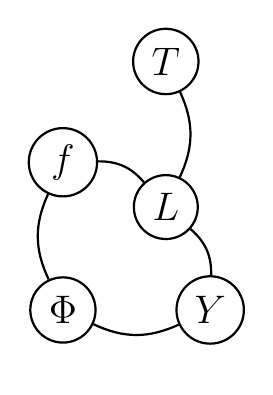
\begin{tikzpicture}[auto, node distance=1cm, every loop/.style={},
			thick,state/.style={circle,draw,font=\sffamily\Large\bfseries}]
			
			
			\node[state] (phi) {$\Phi$};
			\node[state] (f) [above=of phi] {$f$};
			\node[state] (Y) [right =of phi] {$Y$};
			\node[state] (L) [above right =of phi] {$L$};
			\node[state] (T) [above =of L] {$T$};
			
			
			\path (L) edge [bend left = -25] node[below =0.15 cm] {}(T);
			\path (L) edge [bend right = -25] node[below =0.15 cm]  {}(Y);
			\path (L) edge [bend left = -25] node[below =0.15 cm]  {}(f);
			\path (Y) edge [bend right = -25] node[below =0.15 cm]  {}(phi);
			\path (f) edge [bend left = -25] node[below =0.15 cm]  {}(phi);
			\end{tikzpicture}
			\caption{شبکه‌ی مارکوفی متغیّرها در مسئله‌ی طبقه‌بندی}
		\end{figure}
		
		با توجه به این شبکه‌ی مارکوفی و با استفاده از نامساوی پردازش اطّلاعات، می‌توان نوشت:
		
		$$I(T; \bfphi) \leq I(T; \mathbf{Y}) = I(\hat{f}(\mathbf{x}); \mathbf{Y})$$
		
		از طرفی، با توجه به تعریف تابع رشد مجموعه‌ی توابع 
		$\mathcal{F}$
		داریم: 
		\begin{equation}
		I(T;\bfphi) \leq H(T) \leq \log(\Pi_\mathcal{F}(n))
		\label{sa}
		\end{equation}
		با استفاده از لم ساور-شلاح، این عبارت را می‌توان با بُعد 
		\lr{VC}
		مجموعه‌ی 
		$\mathcal{F}$
		که محدود و برابر با 
		$d$
		است، کران‌ زد:
		\begin{equation}
		\Pi_\mathcal{F} (n) \leq
		\begin{cases}
		2^n \;\;\;\;\;\;\; n<d\\
		(\frac{en}{d})^d \;\;\; n\geq d
		\end{cases}
		\label{bo}
		\end{equation}
		
		با ترکیب
		\eqref{sa}
		و
		\eqref{bo}
		داریم:
		$I(\hat{f}(\mathbf{x}), \mathbf{Y}) \leq d \log_+(\frac{en}{d})$.
		
	\end{proof}
	
	
	\subsection{اثبات قضایای فصل
		\ref{randomization}}
	\subsubsection{اثبات لم
		\eqref{lem_randomization}}
	\begin{proof}
		از آن‌جایی که 
		$H_{k} \bigCI T_{k+1}| \phi$،
		با استفاده از نامساوی پردازش اطّلاعات می‌توان نوشت:
		\[
		I(T_{k+1} ; \bfphi) \leq I(H_{k} ; \bfphi).
		\]
		در نتیجه داریم:
		\[
		I( H_k ; \bfphi) = \sum_{i=1}^{k} I\left( (T_i, Y_{T_i}) ; \bfphi |  H_{i-1} \right).
		\]
		لذا
		$I\left( (T_i, Y_{T_i}) ; \bfphi |  H_{i-1} \right)$. Let $\bfphi_{(-i)} = (\phi_{j} : j \neq i)$.
		با این وجود می‌توان نوشت:
		\begin{eqnarray*}
			I\left( (T_i, Y_{T_i}) ; \bfphi |  H_{i-1} \right)&=& I\left( T_i ; \bfphi |  H_{i-1} \right)\\
			&&+ I\left( Y_{T_i} ; \bfphi |  H_{i-1}, T_i \right)\\
			&=& I\left( Y_{T_i} ; \bfphi |  H_{i-1}, T_i \right)\\
			&=& I(Y_{T_i}; \phi_{T_i} | H_{i-1}, T_i )\\
			&&+I(Y_{T_i}; \phi_{(-T_{i})} | H_{i-1}, T_i, \bfphi_{T_i}) \\
			&=& I(Y_{T_i}; \phi_{T_i} | H_{i-1}, T_i ),
		\end{eqnarray*}
		عبارت آخر از استقلال 
		$Y_{T_i}$
		و 
		$ \phi_{(-T_i)}$
		به شرط $\phi_{T_i}$, $Y_{T_i}$ به دست آمده است. به کمک این نامساوی داریم:
		$$I(T_{k+1}; \phi) \leq I(H_k;\phi) = \sum_{i = 1}^{k} I(Y_{T_i};\phi_{T_i}| H_{i-1}, T_i)$$
	\end{proof}


	\end{proof}
	\section{برخی دیگر از کاربردهای مسئله‌ی کاهش سوییدگی از طریق کنترل اطّلاعات استفاده شده}
	\subsection{فیلتر کردن به کمک آماره‌های حاشیه‌ای}
	\label{marginalfiltering}
	
	فرض کنید بعد از مشاهده‌ی دیتاست 
	$D$،
	$T$ 
	انتخاب شده باشد. دیتاست 
	$D$
	مقادیر 
	$\phi_1, \dots, \phi_m$
	را مشخص می‌کند ولی شامل اطّلاعات دیگری نیز هست. داریم:
	\begin{eqnarray}
	I(T; \bfphi) &=& H(T) - H(T| \bfphi) \\
	&\leq& H(T) - I(T;  D |  \bfphi) \\
	&=& (1-\alpha)H(T)
	\end{eqnarray}
	در این معادلات، 
	$\alpha = I(T;D|\bfphi)/H(T)$
	است. این پارامتر، بیانگر کسر عدم قطعیتی است که علاوه بر توابع 
	$\bfphi$
	در  $D$ وجود دارد. در بسیاری از مواقع، 
	$I(T; \bfphi) $
	خیلی کوچک‌تر از 
	$ H(T)$
	است که خود کمتر از 
	$\log(m)$
	می باشد. یک مثال از این سناریو، انتخاب 
	$T$
	بر اساس آماره‌های 
	$D$
	می‌باشد، یک مثال از این مسئله، انتخاب ویژگی مبتنی بر واریانس است. فرض کنید 
	$n$
	نمونه از
	$m$
	ویژگی زیستی در اختیار داریم. مقدار ویژگی $i$ ام در نمونه‌ی 
	$j$
	ام را 
	$X_{i, j}$
	بنامید. دیتاست مورد استفاده
	$D = \{X_{i, j}\}$
	است. تابع 
	$\phi_i$
	را میانگین  نمونه‌ی ویژگی 
	$i$
	ام بگیرید:
	\begin{equation}
	\phi_i = \frac{1}{n}\sum_{j = 1}^{n} X_{i, j}
	\end{equation}
	ما علاقه‌مند به ویژگی‌هایی هستیم که میانگینی به طرز معنادار متفاوت با صفر داشته باشند. برخی از روش‌ها، در ابتدا یک مرحله‌ی  فیلترینگ انجام می‌دهند و تنها ویژگی‌های با واریانس بزرگ را نگه می‌دارند و بقیه را حذف می‌کنند. این فیلترینگ با این استدلال انجام می‌شود که ویژگی‌های با واریانس کم، اطّلاعاتی در بر ندارند و احتمالاً خطای سیستماتیک هستند. سوال طبیعی این است که آیا این فیلترینگ منجر به بایاس می‌شود؟
	
	مسئله‌ را به این صورت فرمول‌بندی می‌کنیم که 
	\begin{equation}
	T = \mathrm{argmax}_i \sum_{j = 1}^{n} (X_{i, j} - \phi_i)^2
	\end{equation}
	یعنی  تنها یک ویژگی انتخاب شده و این ویژگی دارای بزرگترین واریانس می‌یاشد. تمام نتایج امکان تعمیم به حالتی که $k$ ویژگی با واریانس بزرگ انتخاب شده‌اند نیز می‌باشد. قضیه‌ی 
	\eqref{mainthm}
	بیان می‌کند که سوییدگی
	$\E[\phi_T - \mu_T]$
	کوچک است، اگر 
	$I(T; \bfphi)$
	کوچک باشد.
	
	اگر میانگین نمونه و واریانس نمونه خیلی وابسته نباشند، این شرط برقرار می‌شود. به عنوان مثال می‌دانیم که اگر نمونه‌های گاوسی و 
	\lr{i.i.d}
	باشند، 
	$\phi_1, \dots, \phi_m$
	از 
	$V_1,\dots, V_m$
	مستقل  و 
	$I(T; \bfphi) = 0$
	است، در نتیجه  روش سوییدگی ایجاد نمی‌کند.
	
	توجه داشته باشید که در این حالت
	$I(T; D)$
	می‌تواند بسیار بزرگ باشد ولی قضیه‌ی 
	\eqref{mainthm}
	تنها به 
	$I(T; \bfphi)$
	وابسته است. این بدین معناست که انتخاب $T$ تنها وابسته به بخشی از اطّلاعات دیتاست است که در توابع
	$\bfphi$
	خود را نشان نداده است.
	
	در حالت کلّی‌تر این مسئله فرض کنید برای هر ویژگی 
	$i$
	دو آماره‌ی حاشیه‌ای
	$\phi_i$
	و
	$\psi_i$
	محاسبه شده‌اند. بنا بر نامساوی پردازش اطّلاعات داریم
	$I(T; D) \leq I (\mathbf{\psi}; \bfphi)$.
	در این جا 
	$T  = f(\psi_i)$
	است و در تحلیل داده‌، علاقه‌مند به مقادیر
	$\phi_i$
	هستیم و نتیجه‌ی تحلیل ما 
	$\phi_T$
	است.    اگر 
	$\psi_i$
	ها اطّلاعات زیادی از 
	$\phi_i$
	ها در بر نداشته‌باشند، فیلترینگ داده بر اساس‌
	$\psi_i$
	ها منجر به سوییدگی بزرگ نمی‌شود. رابطه‌ی متغیر‌ها در این مسئله به فرم زنجیره‌ی مارکوف
	$T - \mathbf{\psi} - \bfphi$
	مدل می‌شود. با نامساوی پردازش اطّلاعات داریم:
	$I(T; \bfphi) \leq I(\bfphi, \mathbf{\psi}()$
	که منتج به همان نتیجه‌ای که اگر
	$\psi$
	ها و 
	$\phi$
	ها اطّلاعات متقابل کمی داشته باشند، سوییدگی کم است می‌شود. این کران کران تیزی نیست و برای ارائه‌ی یک کران تیز، به نامساوی پردازش اطّلاعات قوی روی‌ می‌آوریم.
	
	\begin{den}
		متغیر‌های تصادفی 
		$X$
		و
		$Y$
		در نامساوی قوی پرازش اطّلاعات با پارامتر 
		$\eta \in [0, 1]$
		صدق می‌کنند، اگر برای هر متغیر تصادفی $U$ با زنجیره‌ی 
		$U-X-Y$
		داشته باشیم:
		$$I(U; Y) \leq \eta I(U;X)$$
		$\eta_{XY}$
		را کوچکترین ضریبی بگیرید که نامساوی فوق برای تمام $U$ ها برقرار باشد.
	\end{den}
	
	یکی از ویژگی‌های جالب ضریب 
	$\eta_{XY}$
	این است که اگر
	$(X_1, Y_1), \dots, (X_n, Y_n)$
	دنباله‌ای مستقل باشد، 
	$\eta_{XY} = \max_i \eta_{X_i Y_i}$
	است. همچنین اگر برای یک متغیر تصادفی 
	$Z$
	زنجیره‌ی 
	$X-Y-Z$
	برقرار باشد،
	$\eta_{XZ} \leq \eta_{YZ}$
	است.
	
	
	\begin{exa}
		فرض کنید 
		$D = (X_1, \dots, X_n)$
		شامل $n$ متغیر تصادفی 
		\lr{i.i.d}
		باشد و 
		$\psi = (X_1, \dots, X_k)$
		که 
		$k \leq n$
		است، یک زیرمجموعه‌ی $n$تایی از آن باشد. در این صورت 
		$\eta_{\psi\phi} \leq \eta_{\psi D} \leq \frac{k}{n}$
		است.
	\end{exa}
	
	توجه داشته باشید که در مثال ما،
	$I_{\psi, \bfphi}$
	تنها تابع توزیع مشترک 
	$\psi$
	و
	$\phi$
	است و ارتباطی با تابع 
	$T = f(\psi)$
	ندارد.  این بدین معناست که از این نامساوی، می‌توان برای ارائه‌ی کرانی تیز بر روی سوییدگی استفاده کرد.
	
	\begin{thm}
		اگر 
		$\phi_i - \mu_i$
		ها متغیرهای تصادفی 
		$\sigma$-زیرگاوسی
		بوده و 
		$T-\psi-\phi$
		برقرار باشد، داریم:
		\begin{equation}
		\E[\phi_T - \mu_T] \leq \sigma \sqrt{2\eta_{\psi\phi} I(T; \psi)}
		\end{equation}
		\begin{proof}
			با توجه به قضیه‌ی 
			\eqref{mainthm}
			و تعریف نامساوی پردازش اطّلاعات قوی، بدیهی است.
		\end{proof}
	\end{thm}


\subsection{استفاده‌کردن از اطّلاعات و مسئله‌ی طبقه‌بندی}
در این بخش به کاربرد قضیه‌ی مطرح‌شده در این مقاله در کران‌زدن خطای جواب مسئله‌ی طبقه‌بندی در یادگیری ماشین می‌پردازیم. فرض کنید
$n$
نمونه‌ی آموزشی در اختیار باشد. هر نمونه، شامل یک بردار 
$X_1, X_2, \dots, X_n \in \mathcal{X}$
است که هر یک به صورت 
\lr{i.i.d.}
از توزیع 
$\mathcal{D}$
انتخاب شده‌اند که توزیع 
$\mathcal{D}$
در اختیار نمی‌باشد. برای هر یک از این 
$n$
نمونه،  متغیر 
$Y_i \in \{0, 1\}$
داده شده است. فرض کنید که برجسب داده‌‌ی
$X_i = x_i$
از توزیع 
$\Prob (Y_i|X_i = x_i)$
گرفته‌شده باشد. 

\begin{den}
	یک طبقه‌بند، تابعی مانند $f$ از 
	$\mathcal{X}$
	به 
	$\{0, 1\}$
	است. خطای یک طبقه‌بند $f$ بدین صورت تعریف می‌شود:
	$$L(f) = \E_{X \sim \mathcal{D}} \left[\mathbf{1}(f(X) \neq Y)\right]$$
	خطای طبقه‌بند بر روی داده‌های آموزشی نیز تعریف می‌شود:
	$$\hat{L}(f)  = \frac{1}{n} \sum_{i = 1}^{n} \mathbf{1} (f(x_i) \neq y_i)$$
	با این تعریف داریم
	$\E[\hat{L}(f)] = L(f)$.
\end{den}

الگوریتم یادگیری ماشین به دنبال تابعی مناسب است که رابطه‌ی بین ویژگی‌ها و برچسب‌ها را مدل کند. هدف این است که تابع
$\hat{f}$
از یک مجموعه‌ی داده‌شده‌ی توابع مثل 
$\mathcal{F}$
است به نحوی  پیدا شود که 
$L(\hat{f}) $
کمینه‌شود. به دلیل اینکه الگوریتم به توزیع 
$\mathcal{D}$
دسترسی ندارد، حل این مسئله‌ی بهینه‌سازی به صورت مستقیم ممکن نیست در نتیجه، به کمک روشی دیگر، تابع 
$\hat{f}$
را انتخاب می‌کنیم. یکی از این روش‌ها، استفاده از 
$$\hat{f} = \mathrm{argmin}_{f \in\mathcal{F}} \hat{L}(f)$$
است. به این الگوریتم
\lr{Empirical Risk Minimization}
یا 
\lr{ERM} 
می‌گویند.


در حالت کلّی، با چنین روش‌هایی ممکن است دچار مشکلی به نام 
\lr{over-fitting}
شویم. این به این معنای این است که با وجود کوچک‌بودن
$\hat{L}(\hat{f})$
مقدار 
$L(\hat{f})$
از 
$\min_{f \in \mathcal{F}} L(f)$
بسیار بزرگ‌تر باشد. تئوری یادگیری ماشین به دنبال بررسی تئوری فاصله‌ی 
$|L(\hat{f}) - \min_{f \in \mathcal{F}} L(f)|$
است. به طور خاص در تئوری یادگیری ماشین، برای الگوریتم‌ها و مجموعه‌های توابع مختلف، به دنبال تابع 
$m_\mathcal{F}$
در تعریف زیر هستند.

\begin{den}
	فرض کنید $m$ نمونه‌ی 
	\lr{i.i.d.}
	$S = \{(X_1, Y_1), (X_2, Y_2), \dots, (X_m, Y_m)\}$
	از توزیع 
	$\mathcal{D}$
	در اختیار باشد. توزیع 
	$\mathcal{D}$
	دلخواه است.  الگوریتم 
	$A$ 
	با دریافت این 
	$m$
	نمونه، تابع 
	$\hat{f} = A_S$
	از مجموعه‌ی توابع
	$\mathcal{F}$
	را انتخاب می‌کند. می‌گوییم مجموعه‌ی توابع 
	$\mathcal{F}$
	توسط الگوریتم
	$A$
	قابل یادگیری به مفهوم 
	\lr{PAC}
	هستند، اگر تابع چند‌جمله‌ای
	$m_\mathcal{F}(., .)$
	وجود داشته‌باشد که به ازای هر 
	$(\epsilon, \delta) \in [0, 1]^2$،
	اگر 
	$m \geq m_\mathcal{F}(\epsilon , \delta)$
	باشد،  با احتمال حداقل 
	$1 - \delta$
	داشته باشیم:
	\begin{equation}
	\E_{X \sim \mathcal{D}} \left[\mathbf{1}(A_S(X) \neq Y) \right]\leq \min_{f \in \mathcal{F}}{\E_{X \sim \mathcal{D}} \left[\mathbf{1}(f(X) \neq Y)\right]} + \epsilon
	\end{equation}
	
	توجه داشته باشید که 
	$m_\mathcal{F}(., .)$
	تنها به مجموعه‌ی 
	$\mathcal{F}$
	ربط دارد و شرط فوق باید به ازای هر توزیع 
	$\mathcal{D}$
	با یک تابع مشخص و ثابت
	$m_\mathcal{F}(., .)$
	برقرار باشد.
	
\end{den}

\begin{exa}
	مثالی از مسئله‌ی طبقه‌بندی این است که 
	$X_i \in \R^d$
	و 
	$\mathcal{F} = \{f_\theta: \theta \in \R^d\}$
	باشد که در آن
	$f_\theta(\mathbf x ) = \mathbf{1}(\mathbf x^\top \theta \geq 0)$
	باشد. الگوریتم $A$ نیز 
	$\theta$
	ای را می‌یابد که در آن 
	$\hat{L}({f_\theta})$
	کمینه‌شود. به این مسئله‌، طبقه‌بندی خطی می‌گوییم. در این مثال، به وضوح می‌دانیم به افزایش 
	$d$
	و با ثابت نگاه داشتن تعداد نمونه‌، ریسک 
	\lr{over-fitting}
	زیاد می‌شود.
\end{exa}

در تئوری یادگیری ماشین، نتایج گوناگونی درباره‌ی کران فاصله‌ی 

$$\left|\E_{X \sim \mathcal{D}} \left[\mathbf{1}(A_S(X) \neq Y)\right] - \min_{f \in \mathcal{F}}{\E_{X \sim \mathcal{D}} \left[\mathbf{1}(f(X) \neq Y)\right]} ‌\right|$$
بر اساس معیار‌های پیچیدگی کلاس 
$\mathcal{F}$
وجود دارد. انتظار داریم با تعداد مشخص نمونه، با افزایش پیچیدگی کلاس 
$\mathcal{F}$،
فاصله‌ی مذکور بزرگ‌تر باشد. یکی از این معیار‌های پیچیدگی، بُعد 
\lr{Vapnik-Chervonenkis}
یا 
\lr{VC Dimension}
است.

\begin{den}
	بُعد 
	\lr{VC}
	مجموعه‌ی توابع 
	$\mathcal{F}$
	برابر بزرگترین کاردینالیتی  مجموعه‌ی 
	$S \subseteq \mathcal{X}$
	است به نحوی که توابع 
	$\mathcal{F}$
	قادر باشند تمام 
	$2^{|S|}$
	برچسب‌گذاری‌ ممکن را بر روی  نمونه‌های آن انجام دهند.
\end{den}

\begin{den}
	تعداد برچسب‌گذاری‌هایی که توابع مجموعه‌ی 
	$\mathcal{F}$
	می‌توانند بر روی یک مجموعه‌ی 
	$S \subseteq \mathcal{X}$
	انجام دهند را با 
	$\Pi_\mathcal{F}(S)$
	نمایش می‌دهیم. تابع رشد مجموعه‌ی توابع 
	$\mathcal{F}$
	به این صورت تعریف می‌شود:
	
	$$\Pi_\mathcal{F}(m) = \max_{S:\;\; |S| = m} \Pi_\mathcal{F} (S)$$
	
	
\end{den}

\begin{lem}
	\textbf {ساور-شلاح}:
	فرض کنید 
	$\mathcal{F}$
	مجموعه‌ای از توابع با بعد 
	\lr{VC}
	محدود 
	$d$
	باشد. در این صورت، به ازای هر 
	$m \in \N$
	داریم:
	\begin{equation}
	\Pi_\mathcal{F}(m) \leq (\frac{em}{d})^d
	\end{equation}
\end{lem}
\begin{proof}
	این قضیه در درس تئوری یادگیری ماشین برای ما اثبات شده است و قضیه‌ی 
	(۳.۵)
	کتاب 
	\cite{mohri2018foundations}
	است.
\end{proof}

\begin{thm}\label{thm_classification}
	فرض کنید 
	$\mathbf{x} = (x_1, \dots x_n)$،
	$\mathbf{Y} = (Y_1, \dots, Y_n)$،
	$\hat{f} (\mathbf{x}) = \big(\hat{f}(x_1), \dots \hat{f}(x_n)\big)$
	و
	$\log_+(z) = \max\{1, \log(z)\}$
	باشند. در این صورت:
	\begin{equation}
	\E[L(\hat{f}) - \hat{L}(\hat{f})] \leq \sqrt{ \frac{I(\hat{f} (\mathbf{x}); Y)}{2n}}
	\label{1}
	\end{equation}
	
	به طور خاص، اگر 
	$\mathcal{F}$
	دارای بعد 
	\lr{VC}
	محدود 
	$d$
	باشد، آن‌گاه
	\begin{equation}
	I(\hat{f} (\mathbf{x}); Y) \leq d \log_+ (\frac{ne}{d})
	\label{2}
	\end{equation}
	
\end{thm}



\begin{cor}
	در تعریف یادگیری
	\lr{PAC}
	دیدیم که برای این نوع یادگیری، نیاز است کرانی ثابت برای تمام توزیع‌های ممکن ورودی به دست آوریم. کران‌های معمول در تئوری یادگیری ماشین نیز از این جنس هستند که مستقل از توزیع ورودی، برای هر توزیع دلخواهی خطا را کران می‌زنند. از طرفی، کران
	\eqref{1}
	وابسته به توزیع داده‌هاست. این نوع کران‌ها می‌توانند منجر به فهم بهتر این مسئله شوند که چه نوع توزیع‌هایی به نحوی بهتر قابل یادگیری هستند. همچنین برای برخی توزیع‌ها،‌کران به دست آمده، می‌تواند بسیار تیز از کران‌های نظریه‌ی 
	\lr{PAC}
	باشد.
\end{cor}



	\subsection{مشاهده‌ی داده‌‌ها و تعداد کلاس‌ها در خوشه‌بندی}
	در بسیاری از مواقع، در مسائل خوشه‌بندی داده‌ها با روش‌هایی مثل 
	\lr{K-Means}،
	شخص پردازش‌گر داده، با مشاهد‌ه‌ی نمودارهای داده، تعداد خوشه‌ها،
	$K$،
	را مشخص می‌کند. در این تحلیل و با توجه به قضیه‌ی
	\eqref{mainthm}،
	سوییدگی ناشی از این کار، اگر 
	$I(T; \phi)$
	کوچک باشد، کم است. بر اساس نامساوی پردازش اطّلاعات داریم:
	$I(T; \bfphi) \leq I(K; \bfphi)$
	است. در مواردی که ساختار مشخضی در داده وجود دارد که الگوریتم خوشه‌بندی قابل درک آن است، معمولاً $K$حول مقادیر خاصی متمرکز است و 
	$I(K; \phi) \leq H(K) \approx 0$
	است. در این مثال، تعداد خوشه‌ها برای تحلیل‌گر داده مفید است ولی مصداق «استفاده‌ی بد از اطّلاعات» نیست.
	\subsection{کنترل سوییدگی از طریق کنترل
		\lr{FDR}
	}
	
	کنترل
	\lr{False Discovery Rate}
	یکی از مسائل مطرح در هنگام انجام تعداد زیاری آزمون‌های فرضیه همزمان است. فرض کنید دیتاست بزرگ 
	$D \in \mathbb{R}^{n\times m}$
	شامل
	$n$
	نمونه از 
	$m$
	ژن باشد. فرض کنید 
	$n_1$
	نمونه‌ی اول از بافتی سرطانی بوده و 
	$n-n_1$
	نمونه‌ی بعدی نیز از بافت سالم آمده باشند. اصولاً دانشمندان علاقه‌مند به یافتن ژن‌هایی هستن که در توده‌ی سرطانی و توده‌های سالم تفاوت معناداری داشته‌باشند. برای این کار، برای هر ژن، یک آزمون فرضیه انجام می‌شود که رد شدن فرضیه‌ی صفر آن، نشان دهنده‌ی این است که بین توزیع این ژن در بافت سرطانی و بافت سالم تفاوت وجود دارد. در این حالت، بسیار نامحتمل است  تفاوت بین ژن در بافت‌های سرطانی و سالم به صورت تصادفی بوده باشد. هدف تنظیم آستانه‌ی رد و قبول فرضیه در این آزمون فرض است.
	
	در این‌جا به بررسی یک حالت بسیار کلّی از این مسئله می‌پردازیم. فرض کنید 
	$D \in \mathbb{R}^{n\times m}$
	یک ماتریس تصادفی بوده و بردار 
	$\phi \in \mathbb{R}^m$
	تابعی از آن باشد. به عنوان مثال، این تابع می‌تواند آماره‌های ستون‌های ماتریس 
	$D$
	باشد، به عنوان مثال، تفاوت میانگین ستون‌ 
	$i$
	ام در بافت‌های سرطانی و بافت‌های سالم.  امید ریاضی این بردار را 
	$\mu$
	بگیرید، یعنی
	$\E \phi(D) = \mu$.
	اندیس‌های 
	$\{1, \dots, m\}$
	به دو بخش 
	$H_0$
	و 
	$H_1$
	تقسیم شده‌اند. یک فرآیند انتخاب، تابعی مثل 
	$\psi: \mathbb{R}^{n\times m} \to \{0, 1\}^m$
	است که 
	$\psi(D)_i  =1$
	نشان می‌دهد که ویژگی (یا ژن) $i$ ام انتخاب شده است. مجموعه‌ی 
	$S_1 \subseteq \{1, \dots, m\}$
	را مجموعه‌ی ژن‌های انتخاب شده و مجموعه‌ی 
	$S_2$
	را مجموعه‌ی ژن‌های انتخاب نشده در نظر بگیرید.  در این فرمول‌بندی، ستون‌های با اندیس عضو
	$H_0$،
	ستون‌هایی هستند که فرض صفر برای آن‌ها برقرار است و تفاوت ژن مربوطه در بافت سالم و سرطانی، معنادار نیست. تعریف‌های زیر، تعریف‌هایی مشابه تعریف های معمول خطای نوع اول و خطای نوع دوم هستند:
	
	$$\hat{\alpha} = \frac{\#(H_0\cap S_1)}{\#H_0} \hspace{2cm} \hat{\beta} = \frac{\#(H_1\cap S_0)}{\#H_1}$$
	
	ما علاقه‌مند هستیم که متغیّر‌هایی به فرم زیر را بررسی کنیم:
	\begin{flalign}
	\frac{1}{\#S_1} \sum_{i \in S_1} (\phi_i - \mu_i)\\
	\frac{1}{\#S_1} \sum_{i \in S_1} |\phi_i - \mu_i|\\
	\frac{1}{\#S_1} \sum_{i \in S_1} (\phi_i - \mu_i)^2
	\end{flalign}
	این متغیر‌ها، به معنای خطا (یا سوییدگی) میانگین در متغیر‌های انتخاب‌شده هستند. این کمیت‌ها را می‌توان به ترتیب به صورت
	$\E[\phi_T - \mu_T]$،
	$\E[\phi_T - \mu_T]$
	و
	$\E[\phi_T - \mu_T]$
	نوشته‌شوند که در آن، متغیر تصادفی 
	$T$
	به شرط
	$D$ 
	دارای توزیع یکنواخت بر روی متغیر‌های انتخاب شده در $S_1$ دارد.
	
	حال،
	\lr{FDR}
	را به صورت
	$\mathrm{FDR} = \mathbf{P}(T \in H_0)$
	تعریف می‌کنیم. این متغیر، نشان می‌دهد که برای چه کسری از متغیر‌های انتخاب شده، عضو 
	$H_0$
	بوده‌اند و اشتباه رخ داده است. قضیه‌ی فوق قضیه‌ای بسیار مهم است که نشان می‌دهد که در صورتی که در فاز آزمون فرضیه و انتخاب ویژگی خوب عمل کنیم و 
	\lr{FDR}
	کوچکی داشته باشیم، اطّلاعات متقابل 
	$I(T;\phi)$
	نیز کوچک است و در نتیجه در فاز تخمین نیز دچار سوییدگی بزرگی نخواهیم بود.
	
	\begin{thm}\label{thm_FDR}
		در مسئله‌ی فوق، داریم:
		\begin{equation}
		I(T;\phi) \leq h(\mathrm{FDR}) + (1-\mathrm{FDR})\log(\frac{1}{1-\beta}) + \mathrm{FDR} \log(\frac{1}{\alpha}) + \xi
		\end{equation}
		که در آن، 
		$h(p)$
		تابع آنتروپی باینری است.
		$\alpha = \E \hat\alpha$
		و
		$\beta = \E \hat\beta$
		خطاهای توع اول و دوم هستند و داریم:
		$$\xi = \E \Big[\log_+(\frac{1-\beta}{1-\hat\beta})\Big] + \E\Big[\log_+(\frac{\alpha}{\hat\alpha})\Big]$$ 
	\end{thm}
	\begin{proof}
		تعریف می‌کنیم
		$\mathcal{X} = \mathbf{1}(T \in H_0)$.
		از آن‌جایی که 
		$\mathcal{X}$
		تابعی یقینی از 
		$T$
		است، می‌توان نوشت:
		\begin{equation}
		I(T;\phi) = I (T; \mathcal{X}, \phi) = I(T;\mathcal{X}) + I(T;\phi|\mathcal{X}) \leq H(\mathcal{X}) + I(T;\phi|\mathcal{X})
		\label{fir}
		\end{equation}
		با استفاده از توزیع 
		$\mathcal{X}$
		و استفاده از نامساوی پردازش اطّلاعات و قاعده‌ی زنجیر، داریم:
		
		\begin{flalign}
		I(T;\phi|\mathcal{X}) &\leq H(\mathcal{X}) + \mathbf{P}(\mathcal{X} = 0) I(T;\phi|\mathcal{X}=0) + \mathbf{P}(\mathcal{X} = 1)I(T;\phi|\mathcal{X} = 1)\\
		&= h\big(\mathbf{P}(T \in H_1)\big) + \mathbf{P}(T\in H_1)I(T;\phi|T\in H_1)\\&+\mathbf{P}(T \in H_0) I(T;\phi|T\in H_0)\\
		&\leq h(\mathbf{P}(T \in H_1)) + \mathbf{P}(T \in H_1) I(T;D|T\in H_1) \\
		&+ \mathbf{P}(T\in H_0) I(T;D|T\in H_0)
		\end{flalign}
		
		می‌توان به سادگی 
		$I(T; D \mid T \in \Hc_1) $
		را به فرم زیر کران زد:
		
		\begin{flalign}
		I(T; D \mid T \in \Hc_1) &= H(T \mid T \in \Hc_1) - H(T| T \in \Hc_1, \,D)\\ 
		&\leq \log( \#\Hc_1 ) - \E[\log\left( \#(S_1 \cap \Hc_1)   \right)  \mid T \in \Hc_1] \\
		&=\log( \#\Hc_1 )- \E[\log\left( (1-\hat{\beta}) \cdot (\#\Hc_1)   \right)  \mid T \in \Hc_1]\\
		&= -\E\left[ \log\left(1-\hat{\beta}  \right) \mid T \in \Hc_1  \right]\\
		&= - \log\left(1-\beta\right) + \E\left[\log\left( \frac{1-\beta}{1-\hat{\beta}}  \right) \, \big\vert \, T \in \Hc_1  \right]
		\end{flalign}
		
		با استفاده از این کران، داریم:
		\begin{flalign}
		\Prob(T \in \Hc_1) I(T; D \mid T \in \Hc_1) &\leq -\Prob(T\in \Hc_1)\log(1-\beta) \\
		&+ \E\left[\log\left( \frac{1-\beta}{1-\hat{\beta}}  \right) \mathbf{1}_{\{T \in \Hc_1\} } \right] \\
		&\leq - \Prob(T\in \Hc_1) \log\left(1-\beta\right) \\
		&+\E\left[\log_{+}\left( \frac{1-\beta}{1-\hat{\beta}}  \right) \right]
		\end{flalign}
		
		با تکرار محاسبات فوق، به نتیجه‌ی زیر می‌رسیم:
		\begin{equation}
		\Prob(T \in \Hc_0) I(T; X \mid T \in \Hc_0) \leq  -\Prob(T\in \Hc_0)\log(\alpha) + \E\left[\log_{+}\left( \frac{\alpha}{\hat{\alpha}}  \right) \right]
		\end{equation}
		
		با جای‌گذاری این نتایج در معادله‌ی 
		\eqref{fir}،
		قضیه اثبات می‌شود.
	\end{proof}
	
	
\end{document}
